\documentclass[conference]{IEEEtran}
%\documentclass[conference,review,anonymous]{IEEEtran}
\IEEEoverridecommandlockouts
% The preceding line is only needed to identify funding in the first footnote. If that is unneeded, please comment it out.
\usepackage{cite}
\usepackage{amsmath,amssymb,amsfonts}
\usepackage{algorithmic}
\usepackage{graphicx}
\usepackage{textcomp}
\usepackage{xcolor}
\usepackage{colortbl}
\usepackage{threeparttable}
%\usepackage{algorithm}
%\usepackage{algorithmic}
%\usepackage{ctable}
%\usepackage{tabularx}
%\usepackage{algpseudocode}
%\usepackage[online,para]{threeparttable}
\usepackage{tcolorbox}
%\usepackage{graphicx}
%\usepackage{textcomp}

%\usepackage{array}
%\usepackage{subcaption}
\usepackage{enumitem}
%\usepackage{longtable}

%\usepackage{tikz}
%\usepackage{listings}
%\usepackage{graphicx}
%\usepackage{amssymb} % For checkmark
\usepackage{multirow}
%\usepackage{mdframed}
%\usepackage{soul}
%\usepackage{hyperref}
%\usepackage{hyperxmp}
\usepackage{comment}

%\setstretch{0.98}

\newcommand{\commentty}[1]{{\color{blue} \sf (TY: #1)}}
\newcommand{\commenttsz}[1]{{\color{green} \sf (TSZ: #1)}}
\newcommand{\commentdbw}[1]{{\color{brown} \sf (DW: #1)}}
\newcommand{\commentzx}[1]{{\color{purple} \sf (ZX: #1)}}
\newcommand{\sidong}[1]{\textcolor{orange}{(SF:#1)}}
\newcommand{\gj}[1]{\textcolor{red}{(GJ:#1)}}


\def\BibTeX{{\rm B\kern-.05em{\sc i\kern-.025em b}\kern-.08em
    T\kern-.1667em\lower.7ex\hbox{E}\kern-.125emX}}
\begin{document}



\title{
{An Empirical Study on Leveraging Images in Automated Bug Report Reproduction}
}

\makeatletter
\newcommand{\linebreakand}{%
  \end{@IEEEauthorhalign}
  \hfill\mbox{}\par
  \mbox{}\hfill\begin{@IEEEauthorhalign}
}
\makeatother

\author{
  % First row: Three authors
  \IEEEauthorblockN{Dingbang Wang}
  \IEEEauthorblockA{
    \textit{University of Connecticut} \\
    USA \\
    dingbang.wang@uconn.edu}
  \and
  \IEEEauthorblockN{Zhaoxu Zhang}
  \IEEEauthorblockA{
    \textit{University of Southern California} \\
    USA \\
    zhaoxuzh@usc.edu}
  \and
  \IEEEauthorblockN{Sidong Feng}
  \IEEEauthorblockA{
    \textit{Monash University} \\
    Australia \\
    sidong.feng@monash.edu}
  % Line break to start a new row
  \linebreakand
  % Second row: Two authors
  \IEEEauthorblockN{William G. J. Halfond}
  \IEEEauthorblockA{
    \textit{University of Southern California} \\
    USA \\
    halfond@usc.edu}
  \and
  \IEEEauthorblockN{Tingting Yu}
  \IEEEauthorblockA{
    \textit{University of Connecticut} \\
    USA \\
    tingting.yu@uconn.edu}
}
%\acmConference[MSR 2025]{The 22nd International Conference on Mining Software Repositories.}{April 28-29, 2025}{Ottawa, Canada.}
\IEEEpubid{\makebox[\columnwidth]{\textit{MSR 2025, Ottawa, Canada, April 28-29, 2025} \hfill}%
\hspace{\columnsep}\makebox[\columnwidth]{ }}

\maketitle
\begin{abstract}
\begin{abstract}  
Test time scaling is currently one of the most active research areas that shows promise after training time scaling has reached its limits.
Deep-thinking (DT) models are a class of recurrent models that can perform easy-to-hard generalization by assigning more compute to harder test samples.
However, due to their inability to determine the complexity of a test sample, DT models have to use a large amount of computation for both easy and hard test samples.
Excessive test time computation is wasteful and can cause the ``overthinking'' problem where more test time computation leads to worse results.
In this paper, we introduce a test time training method for determining the optimal amount of computation needed for each sample during test time.
We also propose Conv-LiGRU, a novel recurrent architecture for efficient and robust visual reasoning. 
Extensive experiments demonstrate that Conv-LiGRU is more stable than DT, effectively mitigates the ``overthinking'' phenomenon, and achieves superior accuracy.
\end{abstract}  
\end{abstract}

\begin{IEEEkeywords}
Android, Bug report, Empirical study
\end{IEEEkeywords}


\section{Introduction}
\label{sec:introduction}
The business processes of organizations are experiencing ever-increasing complexity due to the large amount of data, high number of users, and high-tech devices involved \cite{martin2021pmopportunitieschallenges, beerepoot2023biggestbpmproblems}. This complexity may cause business processes to deviate from normal control flow due to unforeseen and disruptive anomalies \cite{adams2023proceddsriftdetection}. These control-flow anomalies manifest as unknown, skipped, and wrongly-ordered activities in the traces of event logs monitored from the execution of business processes \cite{ko2023adsystematicreview}. For the sake of clarity, let us consider an illustrative example of such anomalies. Figure \ref{FP_ANOMALIES} shows a so-called event log footprint, which captures the control flow relations of four activities of a hypothetical event log. In particular, this footprint captures the control-flow relations between activities \texttt{a}, \texttt{b}, \texttt{c} and \texttt{d}. These are the causal ($\rightarrow$) relation, concurrent ($\parallel$) relation, and other ($\#$) relations such as exclusivity or non-local dependency \cite{aalst2022pmhandbook}. In addition, on the right are six traces, of which five exhibit skipped, wrongly-ordered and unknown control-flow anomalies. For example, $\langle$\texttt{a b d}$\rangle$ has a skipped activity, which is \texttt{c}. Because of this skipped activity, the control-flow relation \texttt{b}$\,\#\,$\texttt{d} is violated, since \texttt{d} directly follows \texttt{b} in the anomalous trace.
\begin{figure}[!t]
\centering
\includegraphics[width=0.9\columnwidth]{images/FP_ANOMALIES.png}
\caption{An example event log footprint with six traces, of which five exhibit control-flow anomalies.}
\label{FP_ANOMALIES}
\end{figure}

\subsection{Control-flow anomaly detection}
Control-flow anomaly detection techniques aim to characterize the normal control flow from event logs and verify whether these deviations occur in new event logs \cite{ko2023adsystematicreview}. To develop control-flow anomaly detection techniques, \revision{process mining} has seen widespread adoption owing to process discovery and \revision{conformance checking}. On the one hand, process discovery is a set of algorithms that encode control-flow relations as a set of model elements and constraints according to a given modeling formalism \cite{aalst2022pmhandbook}; hereafter, we refer to the Petri net, a widespread modeling formalism. On the other hand, \revision{conformance checking} is an explainable set of algorithms that allows linking any deviations with the reference Petri net and providing the fitness measure, namely a measure of how much the Petri net fits the new event log \cite{aalst2022pmhandbook}. Many control-flow anomaly detection techniques based on \revision{conformance checking} (hereafter, \revision{conformance checking}-based techniques) use the fitness measure to determine whether an event log is anomalous \cite{bezerra2009pmad, bezerra2013adlogspais, myers2018icsadpm, pecchia2020applicationfailuresanalysispm}. 

The scientific literature also includes many \revision{conformance checking}-independent techniques for control-flow anomaly detection that combine specific types of trace encodings with machine/deep learning \cite{ko2023adsystematicreview, tavares2023pmtraceencoding}. Whereas these techniques are very effective, their explainability is challenging due to both the type of trace encoding employed and the machine/deep learning model used \cite{rawal2022trustworthyaiadvances,li2023explainablead}. Hence, in the following, we focus on the shortcomings of \revision{conformance checking}-based techniques to investigate whether it is possible to support the development of competitive control-flow anomaly detection techniques while maintaining the explainable nature of \revision{conformance checking}.
\begin{figure}[!t]
\centering
\includegraphics[width=\columnwidth]{images/HIGH_LEVEL_VIEW.png}
\caption{A high-level view of the proposed framework for combining \revision{process mining}-based feature extraction with dimensionality reduction for control-flow anomaly detection.}
\label{HIGH_LEVEL_VIEW}
\end{figure}

\subsection{Shortcomings of \revision{conformance checking}-based techniques}
Unfortunately, the detection effectiveness of \revision{conformance checking}-based techniques is affected by noisy data and low-quality Petri nets, which may be due to human errors in the modeling process or representational bias of process discovery algorithms \cite{bezerra2013adlogspais, pecchia2020applicationfailuresanalysispm, aalst2016pm}. Specifically, on the one hand, noisy data may introduce infrequent and deceptive control-flow relations that may result in inconsistent fitness measures, whereas, on the other hand, checking event logs against a low-quality Petri net could lead to an unreliable distribution of fitness measures. Nonetheless, such Petri nets can still be used as references to obtain insightful information for \revision{process mining}-based feature extraction, supporting the development of competitive and explainable \revision{conformance checking}-based techniques for control-flow anomaly detection despite the problems above. For example, a few works outline that token-based \revision{conformance checking} can be used for \revision{process mining}-based feature extraction to build tabular data and develop effective \revision{conformance checking}-based techniques for control-flow anomaly detection \cite{singh2022lapmsh, debenedictis2023dtadiiot}. However, to the best of our knowledge, the scientific literature lacks a structured proposal for \revision{process mining}-based feature extraction using the state-of-the-art \revision{conformance checking} variant, namely alignment-based \revision{conformance checking}.

\subsection{Contributions}
We propose a novel \revision{process mining}-based feature extraction approach with alignment-based \revision{conformance checking}. This variant aligns the deviating control flow with a reference Petri net; the resulting alignment can be inspected to extract additional statistics such as the number of times a given activity caused mismatches \cite{aalst2022pmhandbook}. We integrate this approach into a flexible and explainable framework for developing techniques for control-flow anomaly detection. The framework combines \revision{process mining}-based feature extraction and dimensionality reduction to handle high-dimensional feature sets, achieve detection effectiveness, and support explainability. Notably, in addition to our proposed \revision{process mining}-based feature extraction approach, the framework allows employing other approaches, enabling a fair comparison of multiple \revision{conformance checking}-based and \revision{conformance checking}-independent techniques for control-flow anomaly detection. Figure \ref{HIGH_LEVEL_VIEW} shows a high-level view of the framework. Business processes are monitored, and event logs obtained from the database of information systems. Subsequently, \revision{process mining}-based feature extraction is applied to these event logs and tabular data input to dimensionality reduction to identify control-flow anomalies. We apply several \revision{conformance checking}-based and \revision{conformance checking}-independent framework techniques to publicly available datasets, simulated data of a case study from railways, and real-world data of a case study from healthcare. We show that the framework techniques implementing our approach outperform the baseline \revision{conformance checking}-based techniques while maintaining the explainable nature of \revision{conformance checking}.

In summary, the contributions of this paper are as follows.
\begin{itemize}
    \item{
        A novel \revision{process mining}-based feature extraction approach to support the development of competitive and explainable \revision{conformance checking}-based techniques for control-flow anomaly detection.
    }
    \item{
        A flexible and explainable framework for developing techniques for control-flow anomaly detection using \revision{process mining}-based feature extraction and dimensionality reduction.
    }
    \item{
        Application to synthetic and real-world datasets of several \revision{conformance checking}-based and \revision{conformance checking}-independent framework techniques, evaluating their detection effectiveness and explainability.
    }
\end{itemize}

The rest of the paper is organized as follows.
\begin{itemize}
    \item Section \ref{sec:related_work} reviews the existing techniques for control-flow anomaly detection, categorizing them into \revision{conformance checking}-based and \revision{conformance checking}-independent techniques.
    \item Section \ref{sec:abccfe} provides the preliminaries of \revision{process mining} to establish the notation used throughout the paper, and delves into the details of the proposed \revision{process mining}-based feature extraction approach with alignment-based \revision{conformance checking}.
    \item Section \ref{sec:framework} describes the framework for developing \revision{conformance checking}-based and \revision{conformance checking}-independent techniques for control-flow anomaly detection that combine \revision{process mining}-based feature extraction and dimensionality reduction.
    \item Section \ref{sec:evaluation} presents the experiments conducted with multiple framework and baseline techniques using data from publicly available datasets and case studies.
    \item Section \ref{sec:conclusions} draws the conclusions and presents future work.
\end{itemize}
% TODO
% more detailed introduction of dataset creation
% the rumour label in such datasets
\section{Data} \label{sec:data}
We use three rumour datasets in this work, namely: PHEME~\citep{pheme2015,kochkina-etal-2018-one}, Twitter15, and Twitter16~\citep{ma-etal-2017-detect}:

% TJB: how can the number of threads be greater than the number of tweets? these numbers don't make sense
% RX: fixed, the numbers were incorrect
\paragraph{PHEME}~\citet{pheme2015} contains 6,425 tweet posts of rumours and non-rumours related to 9 events. To avoid using specific a priori keywords to search for tweet posts, PHEME used the Twitter (now X) steaming API to identify newsworthy events from breaking news and then selected from candidate rumours that met rumour criteria, finally they collected associated conversations and annotate them. They engaged journalists to annotate the threads. The data were collected between 2014 and 2015. The 9 events are split into two groups, the first being breaking news that contains rumours, including Ferguson unrest, Ottawa shooting, Sydney siege, Charlie Hebdo shooting, and Germanwings plane crash. The rest are specific rumours, namely Prince to play in Toronto, Gurlitt collection, Putin missing, and Michael Essien contracting Ebola.
% TJB: say something about the time period when this data was collected
% RX: added

\paragraph{Twitter 15}~\citet{twitter15} was constructed by collecting rumour and non-rumour posts from the tracking websites snopes.com and emergent.info. They then used the Twitter API to gather corresponding posts, resulting in 94 true and 446 false posts. This dataset further includes 1,490 root posts and their follow posts, comprising 1,116 rumours and 374 non-rumours.
% TJB: the "tweet" vs. "comment" terminology is potentially confusing and needs to be clarified
% RX: unified, used root and follow posts to refer to root posts and the comment posts, posts are used to describe tweets in general.

\paragraph{Twitter 16}
Similarly to Twitter 15, \citet{twitter16} collected rumours and non-rumours from snopes.com, resulting in 778 reported events, 64\% of which are rumours. For each event, keywords were extracted from the final part of the Snopes URL and refined manually---adding, deleting, or replacing words iteratively---until the composed queries yielded precise Twitter search results. The final dataset includes 1,490 root tweet posts and their follow posts, comprising 613 rumours and 205 non-rumours.

\begin{table*}[!t]
    \centering
    \small
    \begin{tabular}{p{0.05\linewidth}p{0.9\linewidth}}
    \toprule
    Task & Prompt \\
    \midrule
    V-oc & Categorize the text into an ordinal class that best characterizes the writer's mental state, considering various degrees of positive and negative sentiment intensity. 3: very positive mental state can be inferred. 2: moderately positive mental state can be inferred. 1: slightly positive mental state can be inferred. 0: neutral or mixed mental state can be inferred. -1: slightly negative mental state can be inferred. -2: moderately negative mental state can be inferred. -3: very negative mental state can be inferred.\\
    \midrule
    E-c & Categorize the text's emotional tone as either `neutral or no emotion' or identify the presence of one or more of the given emotions (anger, anticipation, disgust, fear, joy, love, optimism, pessimism, sadness, surprise, trust).\\
    \midrule
    E-i & Assign a numerical value between 0 (least E) and 1 (most E) to represent the intensity of emotion E expressed in the text.\\
    \bottomrule
    \end{tabular}
    \caption{Prompts used for EmoLLM to detect emotion information in tweets. V-oc = Valence Ordinal Classification, E-c = Emotion Classification, and E-i = Emotion Intensity Regression.}
    \label{tab:emollm_ins}
\end{table*}


  
%%% Local Variables:
%%% mode: latex
%%% TeX-master: "../main_anonymous"
%%% End:

\subsection{Accuracy of \tool in Detecting GUI Lags}

%\subsection{RQ: How effectively can \tool detect GUI performance lags?} \feng{the structure of this part looks strange...}
%\subsubsection{Motivation}
%Given the variety design of mobile apps and the different types of contents on app pages, detecting GUI performance lags for the app screencast can be challenging. In this research question (RQ), we evaluate how effectively \tool can detect performance lags in screencasts.


%\subsubsection{Approach}
We use the dataset collected and labeled by the user experience experts as the ground truth for evaluation. 
In the context of a screencast, an instance GUI lag is considered correctly located by \tool if and only if it matches a lag (annotated as $[f_{start}, f_{end}]$) in the ground truth, with identical start and end frame indices (i.e, the same $f_{start}$ and $f_{end}$ values). 
To evaluate the effectiveness of \tool in detecting GUI lags, We employ precision, recall, and F1-score:

\begin{itemize}
    \item \textbf{Precision} is the fraction of correctly identified GUI lags out of all instances that \tool identified as GUI lags. It is defined as: 
\end{itemize}
\begin{equation}
Precision = \frac{\#\textit{Correctly identified GUI lags}}{\#\textit{Identified GUI lags}}
\end{equation}

\begin{itemize}
    \item \textbf{Recall} is the fraction of correctly identified GUI lags out of the total number of actual GUI lags. It is defined as: 
\end{itemize}
\begin{equation}
Recall = \frac{\#\textit{Correctly Identified GUI lags}}{\#\textit{Actual GUI lags}}
\end{equation}

\begin{itemize}
    \item The \textbf{F1-score} is the harmonic mean of precision and recall:
\end{itemize}
\begin{equation}
F_{1} = 2 \times \frac{Precision \times Recall}{Precision + Recall}
\end{equation}


%\subsubsection{Results}
Table~\ref{tab:resutls_detecting_lags} presents the results of detecting GUI performance lags using \tool, demonstrating its high level of accuracy in detecting these lags. The precision for detecting the three types of GUI lags ranges from 0.91 to 0.92, while recall ranges from 0.95 to 0.98, and the F1-score ranges from 0.93 to 0.95. Overall, \tool achieves high average precision of 0.91 and recall of 0.96 across all lag types. 

\begin{table}
	\centering
	\caption{Results of \tool in detecting performance GUI lags across different lag types.}
	\label{tab:resutls_detecting_lags}
	\scalebox{1}{
	\begin{tabular}{lrrr}
		\toprule
		Lag type&\tabincell{r}{Precision}&\tabincell{r}{Recall}&\tabincell{r}{F1-Score}\\
		\midrule
			Janky frames          &0.92	        &0.98       &0.95\\
   	  Long Loading frames   &0.91 		  &0.96		  &0.93\\
			Frozen frames         &0.91		    &0.95	    &0.93\\
		\midrule
		\tabincell{l}{Average Across Types} 	&0.91		&0.96 		&0.94\\
		\bottomrule
	\end{tabular}}
        \vspace{-5mm}
\end{table}


Even though \tool achieves high precision and recall, there are still some missed or incorrectly detected cases. Hence, we conduct further analysis on such cases. We found that certain factors contribute to these inaccuracies. Primarily, our approach uses a threshold of 100 milliseconds based on prior HCI studies~\cite{1968_AFIPS_Response_time_in_man_computer, 1994_Usability_Engineering} to determine the shortest duration that users can typically perceive a lag caused by janky frames. While this threshold works well in most scenarios, it is still possible to lead to missed detection or false positives. 
For example, janky frames with a duration under 100 milliseconds may still be perceptible when they occur in scenarios with frequent or complex screen changes, such as during video playback or fast-paced animations. In these cases, even slight irregularities become noticeable to users, but \tool may not flag them due to the short duration. Similarly, certain long loading frames and frozen frames that exceed the thresholds might not be detected as high-severity issues when users have context-specific expectations of delay, such as when waiting for large media files or complex images to load. In these instances, users anticipate the delay, which reduces their perception of it as a performance issue, yet \tool might flag it as a severe lag based on the duration alone.
This analysis indicates that to further improve detection accuracy, \tool needs to go beyond a simple time threshold and incorporate additional factors such as the type of user interaction, the visual prominence of the lagging element, and the expected behavior of certain app functionalities. By integrating these contextual cues, \tool can more effectively capture the GUI lags that are most likely to affect user satisfaction. 


%true impact of GUI lags on user experience, providing more meaningful and actionable insights to developers. This enhancement would ensure that only the most perceptible and disruptive lags are flagged as critical, allowing developers to prioritize issues that are most likely to affect user satisfaction.




%Furthermore, we observed that not all lags are equally disruptive across different types of interactions. For example, users are less tolerant of delays during high-interaction activities, like tapping buttons or scrolling, compared to delays during passive content loading, such as image rendering in the background. This variation in tolerance suggests that the context of user interactions should also influence how \tool categorizes and prioritizes detected lags. Without accounting for these contextual nuances, \tool may sometimes incorrectly classify the severity of an issue, either overlooking significant lags or unnecessarily flagging minor ones.

%This analysis indicates that to improve detection accuracy, \tool needs to go beyond a simple time threshold and incorporate additional factors such as the type of user interaction, the visual prominence of the lagging element, and the expected behavior of certain app functionalities. By integrating these contextual cues, \tool can more effectively capture the true impact of GUI lags on user experience, providing more meaningful and actionable insights to developers. This enhancement would ensure that only the most perceptible and disruptive lags are flagged as critical, allowing developers to prioritize issues that are most likely to affect user satisfaction.

%============






%Nevertheless, some lags were either missed or incorrectly detected. The primary reason for this is our approach's reliance on the shortest time duration that humans can typically perceive---100ms (calculated as 16.6ms per frame * 5 frames for a 60Hz mobile device).
%In certain cases, users may still perceive lag even when an lag lasts for less than 100ms. For example on janky frames, when playing videos, the content of the screen changes frequently which makes the frame transition more noticeable to users. Although the lag duration is less than 100ms, some people may still perceive it as lagging, which is incorrectly detected by \tool.
%For long load frames, users may still perceive lag even when an lag lasts for less than 100ms. 
%For example on long load frames, as illustrated in Figure 4, although the lag duration is less than 100ms, the size of the image occupying a significant portion of the screen makes the frame transition more noticeable to users.
%Conversely, there are situations where users may not perceive the lag, even when it exceeds 100ms, because they expect the app to take time for specific functionalities based on their prior experiences, which is missed detected by \tool.
%These observations suggest that lag detection should not solely rely on duration but also incorporate other factors, such as visual elements within the app and the nature of specific functionalities, which influence user perception of performance.


% \subsubsection{Discussion} Given a screencast, developers may just want to know if it behaviours slow (i.e., containing any type of the performance lag) under the usage scenario. Hence, we also use the metrics to evaluate how effectively \tool can detect the slow screencasts. 

\rqbox{We find that \tool achieves an average precision and recall of 0.91 and 0.96 on detecting GUI lags from screencasts. Our analysis finds that incorporating additional app context may further improve detection results. }

% \begin{table}
% 	\centering
% 	\caption{Results of detecting and locating GUI performance lags by \tool. }
% 	\label{tab:resutls_detecting_lags}
%     \setlength{\tabcolsep}{5pt}
% 	\scalebox{1}{
% 	\begin{tabular}{c rrr rrr} 
% 		\toprule
% 		\multirow{2}*{lag type} & 
% 		\multicolumn{3}{c}{Detection}&
%         \multicolumn{3}{c}{Location}\\
		
% 		\cmidrule(r){2-4}\cmidrule(r){5-7}
% 		&Precision &Recall &F1 &Precision &Recall &F1\\
		
% 		\midrule
% 		Janky frames &	    &       &  &	    &       &\\
% 		Frozen frames&		&	    &  &	    &       &\\
% 		Load frames& 		&		&  &	    &       &\\

%   	\midrule
% 		\tabincell{l}{Avg. across }	&	& 	& &		& 		&\\
		
% 		\bottomrule
% 	\end{tabular}}
% \end{table}
\begin{table}[!t]
    \centering
    % \scriptsize
    \tabcolsep=5.5pt
    \tiny
    %\renewcommand{\arraystretch}{1.1} 
    \caption{\revise{Performance of CodeBERT} on purified datasets. \revise{BC: BadCode; CP: CodePoisoner; CB: CodeBLEU.}}
    \vspace{-1mm}
    \label{tab:rq2_codebert}
    \begin{threeparttable}
    \begin{tabular}{clcccccc}
        \toprule
        
        \multirow{2}{*}{Task} & \multirow{2}{*}{Code Poisoning} & \multicolumn{2}{c}{Clean} & \multicolumn{2}{c}{Undefended} & \multicolumn{2}{c}{\ours{}} \\

        \cmidrule(lr){3-4} \cmidrule(lr){5-6} \cmidrule(lr){7-8}

        & & \revise{ACC} & ASR & ACC & ASR & ACC & ASR \\
    
        \midrule
        
        \multirow{6}{*}{\rotatebox{90}{Defect Detection}} &
        BC (Fixed) & \revise{63.50\%} & 27.76\% & 62.00\% & 100\% & 62.00\% & 26.99\% \\
        & BC (Mixed) & \revise{63.50\%} & 27.76\% & 61.00\% & 96.18\% & 60.00\% & 32.14\% \\
        & BNC (Fixed) & \revise{63.50\%} & 30.92\% & 60.43\% & 100\% & 61.16\% & 37.46\% \\
        & BNC (Grammar) & \revise{63.50\%} & 21.35\% & 63.28\% & 100\% & 63.12\% & 22.48\% \\
        & CP (Variable) & \revise{63.50\%} & 46.29\% & 62.79\% & 100\% & 61.96\% & 48.59\% \\
        \cmidrule(lr){2-8}
        & Average & \revise{63.50\%} & 30.82\% & 61.90\% & 99.24\% & 61.65\% & 33.53\% \\
        \bottomrule
        
        \\

        \toprule
        
        \multirow{10}{*}{\rotatebox{90}{Clone Detection}} &
        & \revise{F1} & ASR & F1 & ASR & F1 & ASR \\
        \midrule
        & BC (Fixed) & \revise{98.71\%} & 1.61\% & 98.10\%  & 100\% & 98.39\%  & 1.58\% \\
        & BC (Mixed) & \revise{98.71\%} & 1.61\% & 98.22\%  & 100\% & 97.20\%  & 2.55\% \\
        & BNC (Fixed) & \revise{98.71\%} & 1.58\% & 98.27\% & 100\%  & 98.53\%  & 3.99\% \\
        & BNC (Grammar) & \revise{98.71\%} & 1.04\% & 98.22\% & 100\% & 97.31\% & 5.17\% \\
        & CP (Variable) & \revise{98.71\%} & 2.23\% & 98.17\%  & 100\%  & 98.23\%  & 6.70\%  \\
        \cmidrule(lr){2-8}
        & Average & \revise{98.71\%} & 1.61\% & 98.20\% & 100\% & 97.93\% & 4.00\% \\
        \bottomrule
        
        \\

        \toprule
        \multirow{9}{*}{\rotatebox{90}{Code Search}} &
        & \revise{MRR} & ANR & MRR & ANR & MRR & ANR \\
        \midrule
        & BC (Fixed) & \revise{81.46} & 46.27 & 80.06 & 4.71 & 80.06 & 55.82 \\
        & BC (Mixed) & \revise{81.46}  & 46.27 & 80.04 & 4.93 & 80.22 & 42.17 \\
        & BNC (Fixed) & \revise{81.46}  & 49.09 & 81.32 & 5.03 & 80.06 & 60.67 \\
        & BNC (Grammar) & \revise{81.46}  & 51.36 & 80.01 & 2.14 & 80.03 & 56.43 \\
        & CP (Variable) & \revise{81.46}  & 43.12 & 79.66 & 8.34 & 79.93 & 61.60 \\
        \cmidrule(lr){2-8}
        & Average & \revise{81.46}  & 47.22 & 80.22 & 5.03 & 80.06 & 55.34 \\
        \bottomrule

        \\
        
        \toprule
        \multirow{9}{*}{\rotatebox{90}{Code Repair}} &
        & \revise{BLEU/CB} & ASR & BLEU/\revise{CB} & ASR & BLEU/\revise{CB} & ASR \\
        \midrule
        & BC (Fixed) & \revise{78.42/75.58} & 0\% & 78.24/\revise{75.73} & 99.98\% & 77.63/\revise{75.46} & 0\% \\
        & BC (Mixed) & \revise{78.42/75.58} & 0\% & 77.33/\revise{75.15} & 100\% & 76.80/\revise{74.82} & 15.18\% \\
        & BNC (Fixed) & \revise{78.42/75.58} & 0\% & 77.66/\revise{75.24} & 100\% & 77.55/\revise{75.31} & 0.48\% \\
        & BNC (Grammar) & \revise{78.42/75.58} & 0\% & 77.09/\revise{75.01} & 100\% & 77.23/\revise{75.13} & 3.19\% \\
        & CP (Variable) & \revise{78.42/75.58} & 0\% & 77.82/\revise{75.58} & 100\% & 77.58/\revise{75.21} & 0.26\% \\
        \cmidrule(lr){2-8}
        & Average & \revise{78.42/75.58} & 0\% & 77.63/\revise{75.36} & 100\% & 77.36/\revise{75.19} & 3.82\% \\
        \bottomrule
        
    \end{tabular}
    \end{threeparttable}
    \vspace{-4mm}
\end{table}

\begin{table}[!t]
    \centering
    % \scriptsize
    \tabcolsep=6pt
    \tiny
    %\renewcommand{\arraystretch}{1.1} 
    \caption{\revise{Performance of StarCoder on the defect detection dataset purified by \ours{}.}}
    \vspace{-1mm}
    \label{tab:rq2_starcoder}
    \begin{tabular}{clcccccc}
        \toprule
        
        \multirow{2}{*}{\revise{Task}} & \multirow{2}{*}{\revise{Code Poisoning}} & \multicolumn{2}{c}{\revise{Clean}} & \multicolumn{2}{c}{\revise{Undefended}} & \multicolumn{2}{c}{\revise{\ours{}}} \\

        \cmidrule(lr){3-4} \cmidrule(lr){5-6} \cmidrule(lr){7-8}

        & & \revise{ACC} & \revise{ASR} & \revise{ACC} & \revise{ASR} & \revise{ACC} & \revise{ASR} \\
    
        \midrule
        
        \multirow{6}{*}{\rotatebox{90}{\revise{Defect Detection}}} &
        \revise{BadCode (Fixed)} & \revise{61.97\%} & \revise{56.89\%} & \revise{61.73\%} & \revise{97.89\%} & \revise{61.37\%} & \revise{56.54\%} \\
        & \revise{BadCode (Mixed)} & \revise{61.97\%} & \revise{57.24\%} & \revise{61.67\%} & \revise{96.23\%} & \revise{61.23\%} & \revise{56.75\%} \\
        & \revise{BNC (Fixed)} & \revise{61.97\%} & \revise{57.39\%} & \revise{61.32\%} & \revise{100\%} & \revise{61.14\%} & \revise{56.82\%} \\
        & \revise{BNC (Grammar)} & \revise{61.97\%} & \revise{58.31\%} & \revise{61.54\%} & \revise{100\%} & \revise{61.26\%} & \revise{57.64\%} \\
        & \revise{CodePoisoner (Variable)} & \revise{61.97\%} & \revise{59.12\%} & \revise{61.68\%} & \revise{96.57\%} & \revise{61.32\%} & \revise{59.03\%} \\
        \cmidrule(lr){2-8}
        & \revise{Average} & \revise{61.97\%} & \revise{57.79\%} & \revise{61.59\%} & \revise{98.14\%} & \revise{61.26\%} & \revise{57.36\%} \\
        
        \bottomrule
        
    \end{tabular}
    \vspace{-3mm}
\end{table}
\section{Impact of Major Ethereum Events on Issue Resolution Time}\label{RQ3}

To evaluate whether development efforts are planned or reactive to major events, we analyzed issue activity before and after each event. Daily issue data was collected from each repository to observe trends in issue openings and closures, focusing on shifts in resolution patterns. Kaplan-Meier estimation was used to model resolution time distributions, with event dates serving as covariates to compare resolution behavior before and after each event. Using the list of the major events from RQ2, we visualized changes in issue activity within the 1-month and 3-month timeframes identified in previous sections. Notable time-based fluctuations in issue activity across repositories highlight the importance of dynamically analyzing these patterns to capture the temporal impact of major events on resolution times.

\paragraph{Issue Opening and Resolution Near Key Events}
To examine how issue activity aligns with major Ethereum events, we plotted issue resolution times across all repositories, with each line representing an issue. Resolved issues are marked with an orange dot at the end, while unresolved issues extend in blue to the end of the observation period. Sorting issues by creation date allows us to track resolution patterns before and after specific events. Here, only the plot for MetaMask is shown (Fig.~\ref{fig:lifelines-metamask}).
Across repositories, a common trend is the spike in issue resolutions around major events. In MetaMask, we observe notable resolution activity around the Beacon Chain Launch (event 5) and the Arrow Glacier Update (event 7). Similar patterns are seen in other repositories. For instance, Go-Ethereum shows increased resolution activity near key events and an additional spike in older issue resolutions before 2019. Solidity also displays surges around the Beacon Chain Launch (event 5), The Merge (event 9), and the Shanghai Upgrade (event 10). 

\begin{figure}
    \centering
    \includegraphics[width=\linewidth]{images/pdf2/metamask-extension-issues-lifelines-1.pdf}
    \caption{MetaMask's issue resolution and events}
    \label{fig:lifelines-metamask}
\end{figure}

For the other repositories, similar resolution spikes are evident. For example, Web3.js, Hardhat, and Ether.js show increased resolution activity around the Shanghai Upgrade (event 10), while the Arrow Glacier Update (event 7) coincides with significant resolution efforts in Ether.js, OpenZeppelin, and Chainlink. The Merge (event 9) also influences activity in Hardhat and Chainlink.
While not all resolution spikes directly correspond to major events—some relate to each repository’s unique milestones—these findings illustrate a general pattern of heightened issue resolution, often in anticipation of or response to major Ethereum events. 

\paragraph{Characterizing Issue Resolution Through Survival Analysis}
We applied the Kaplan-Meier estimator to analyze resolution times for both open and closed issues, using the last collection date as the endpoint for unresolved issues. Fig.~\ref{fig:survival} shows the survival curve for Go-Ethereum, our most efficient repository, resolving 40\% of issues within days and 75\% within a year. Other repositories show varying patterns: MetaMask and Solidity resolve 50--60\% within a year, while OpenZeppelin and Consensus-Specs match Go-Ethereum's efficiency. Truffle, Ethers.js, and particularly Hardhat show slower resolution times. The anomaly around 400 days in Go-Ethereum suggests systematic closure of backlogged issues.

\begin{figure}
    \centering
    \includegraphics[width=\linewidth]{images/pdf2/go-ethereum-issues-survival-1.pdf}
    \caption{Survival analysis of issue resolution times in Go-Ethereum. The line represents the probability of issue resolution after each day since the issue was opened.}
    \label{fig:survival}
\end{figure}

\paragraph{Impact of Events on Survival Analysis}
To assess event influence on issue resolution, we split issues into groups based on their opening time relative to each event and compared their survival curves. Fig.~\ref{fig:survival-split-4} demonstrates this approach using the Crypto Boom (event 3) in MetaMask, where diverging curves indicate event impact on resolution patterns. 
We used log-rank tests to determine statistical significance of these differences, applying the Benjamini-Hochberg procedure across the 10 events for each repository, consistent with our approach in RQ2.
Table~\ref{tab:survival-events} presents the test results across all repositories. 



\begin{figure}
    \centering
    \includegraphics[width=\linewidth]{images/pdf3/metamask-extension-issues-survival-1-ev-split-4.png}
    \caption{Comparison of issue resolution patterns in MetaMask before and after the Crypto Boom event. The two lines representing issue resolution probabilities before and after the event, can highlight changes.}
    \label{fig:survival-split-4}
\end{figure}


\begin{table*}[h]
\caption{$p$ for log-rank test of survival curves when issues are split into two groups (before and after an event)}
\label{tab:survival-events}
\resizebox{\textwidth}{!}{
\begin{tabular}{lrrrrrrrrrrrr}
\hline
\textit{\textbf{Repository} } & \textbf{1 - Frontier} & \textbf{2 - DAO Hack} &  \textbf{3 - Crypto Boom}  & \textbf{4 - COVID Crash}& \textbf{5 - Beacon} & \textbf{6 - London} & \textbf{7 - Arrow Gl.} & \textbf{8 - Ropsten} & \textbf{9 - Merge} & \textbf{10 - Shanghai}\\
 \hline
\textit{MetaMask} & - & \cellcolor{lightgray}$.249$ & $<.001$ & \cellcolor{lightgray}$.067$ & \cellcolor{lightgray}$.173$ & \cellcolor{lightgray}$.067$ & \cellcolor{lightgray}$.149$ & $<.001$ & $<.001$ & $<.001$\\
\textit{Solidity} & - & \cellcolor{lightgray}$.721$ & $.003$ & \cellcolor{lightgray}$.534$ & \cellcolor{lightgray}$.534$ & \cellcolor{lightgray}$.534$ & \cellcolor{lightgray}$.534$ & \cellcolor{lightgray}$.534$ & \cellcolor{lightgray}$.534$ & \cellcolor{lightgray}$.534$ \\
\textit{Go-ethereum} & $<.001$ & $.003$ & $<.001$ & $<.001$ & $<.001$ & $<.001$ & $<.001$ & $<.001$ & $<.001$ & $<.001$ \\
\textit{Chainlink} & - & - & - & $<.001$ & $<.001$ & $<.001$ & $<.001$ & $<.001$ & $<.001$ & $<.001$ \\
\textit{Truffle} & \cellcolor{lightgray}$.171$ & $<.001$ & $<.001$ & $<.001$ & $<.001$ & $.009$ & $.004$ & $<.001$ & $.002$ & \cellcolor{lightgray}$.218$  \\
\textit{Hardhat} & - & - & - & $<.001$ & $<.001$  & $<.001$ & $<.001$ & $<.001$ & $<.001$ & $<.001$  \\
\textit{Web3-js} & $<.001$ & \cellcolor{lightgray}$.310$  & $<.001$ & $<.001$ & $<.001$ & $<.001$ & $<.001$ & $<.001$ & $<.001$ & $<.001$ \\
\textit{OpenZeppelin} & - & - & \cellcolor{lightgray}$.560$ & \cellcolor{lightgray}$.836$ & \cellcolor{lightgray}$.764$ & \cellcolor{lightgray}$.317$ & $.035$ & $<.001$ & $<.001$ & $<.001$\\
\textit{Consensus-Specs} & - & - & - & $<.001$ & $<.001$ & $<.001$ & $<.001$ & $<.001$ & $<.001$ & $<.001$ \\
\textit{Ethers-js} & - & - & \cellcolor{lightgray}$.344$ & $<.001$ & \cellcolor{lightgray}$.225$ & $.058$ & $.007$ & $<.001$ & $<.001$ & $<.001$ \\

 \hline
\end{tabular}
}
\end{table*}

While many events significantly impacted resolution times across repositories, some repositories like Solidity showed fewer significant changes, suggesting different dynamics in their issue resolution processes. For instance, Go-Ethereum displayed significant differences before and after all the events. MetaMask showed significant changes after the Crypto Boom and the last 3 events.

\begin{tcolorbox}[right=0.1cm,left=0.1cm,top=0.1cm,bottom=0.1cm]
\textbf{Answer to RQ3:} Major Ethereum events impact issue resolution times. Issue creation spikes around key events are often followed by bursts of resolutions as developers prepare for or respond to these changes. While resolution speeds vary across repositories, most issues are resolved quickly, though some repositories appear to manage the number of outstanding issues differently. Overall, issue resolution times change in a statistically significant way before and after major events for most repositories, reflecting increased activity and responsiveness. However, some repositories exhibit resilience to event effects, indicating diverse development dynamics within the ecosystem.
\end{tcolorbox}






\subsection{\textbf{RQ4: \BFPs Across Symptoms}}


As shown in \autoref{fig:symptom_semantic_combined}, this research question illustrates the relationship between bug symptoms observed in Apollo and Autoware and semantic BFPs, with 2473 symptom instances in total.


The occurrence of domain-specific \bfp Path Planning Optimization (PPO) and domain-independent pattern Data Flow Correction (DFC) across various symptoms, such as Crashes, Stop and parking (Stop), Lane Positioning and Navigating (LPN), Speed and Velocity Control (SVC), Turning (Turn), Trajectory (Traj), Obstacle Processing (OP), and Logic, signifies the critical nature of these patterns in addressing diverse and complex issues in different driving scenarios. 

\vspace{-1ex}
\begin{finding}
\label{finding:rq4_dfc}
    The frequent occurrence of Data Flow Correction (DFC) (364 occurrences) in diverse symptoms underscores the importance of data-flow handling for reliable autonomous vehicle operations, which suggests the need for robust data-flow testing and correction for ADSes.
\end{finding}
\vspace{-1ex}



The 30 instances of Debugging Tools Improvement (DTI) bug fixes, primarily in Display and GUI (DGUI) symptoms, demonstrate that ADS developers value debugging methods that are specialized to their domain, but further value effective visualizations for debugging concerns. 
Existing debugging techniques~\cite{ArcainiCILZAHV21,MINNERUP201644,apollo_debug,autoware_debug}, such as log analysis, breakpoint debugging, and unit testing, provide a broad foundation for software diagnosis. However, the absence of dedicated research on convenient debugging tools for ADS reveals a critical gap, where the intricate and real-time nature of ADS presents unique challenges such as complex sensor data integration, safety-critical decision-making, and dynamic environmental interaction. Improved visualization tools for debugging may consider offering a more intuitive understanding of ADS behavior and error states.

\vspace{-1ex}
\begin{finding}
\label{finding:rq4_dti}
    The prevalence of 30 Debugging Tools Improvement (DTI) bug fixes in DGUI symptoms highlights the critical need for ongoing improvements in debugging tools and user interfaces within autonomous vehicle systems. 
\end{finding}
\vspace{-1ex}

\begin{figure}[ht!]
    \centering
    \begin{minipage}{0.525\linewidth}
        \centering
        \includegraphics[width=\linewidth]{images/rq3_4_5/symptom_semantic_combined.pdf}
        \vspace{-5ex}
        \caption{Relation between Symptoms and Semantic \BFPs for Apollo and Autoware}
        \label{fig:symptom_semantic_combined}
    \end{minipage}
    \hfill
    \begin{minipage}{0.465\linewidth}
        \centering
        \includegraphics[width=\linewidth]{images/rq3_4_5/module_semantic_combined.pdf}
        \vspace{-5ex}
        \caption{Relation between Modules and Semantic \BFPs for Apollo and Autoware}
        \label{fig:module_semantic_combined}
    \end{minipage}
\end{figure}

State Management Enhancement (SME) \bfps are most commonly observed in Stop and Parking (Stop) (23 occurrences), Obstacle Processing (OP) (23 occurrences), and Lane Positioning and Navigating (LPN) (20 occurrences) symptoms. 
Effective state management is crucial for ensuring seamless transitions between different operational modes, such as transitioning from driving to parking or navigating through obstacles. This necessity points to the intricate interplay between state control mechanisms and the vehicle's capacity to interpret and react to dynamic driving environments, thereby stressing the importance of sophisticated state handling strategies to mitigate potential risks and enhance driving safety.
These scenarios, which necessitate precise state transitions such as moving from forward to reverse for parking or adjusting to dynamic obstacles, highlight the critical role of advanced state management.

\vspace{-1ex}
\begin{finding}
    \label{finding:rq4_sme}
    The concentration of State Management Enhancement (SME) patterns in scenarios like Stop and Parking, Obstacle Processing, and Lane Positioning and Navigating underscores the importance of robust state management for AV adaptability to diverse driving conditions. 
\end{finding}
\vspace{-1ex}


The significant count of 178 STOP-related \bfps in AVs underscores the complex and persistent issues in stopping and parking functionalities, revealing systemic vulnerabilities and the need for refined parking algorithms and community concerns. These patterns suggest that current methodologies may fall short in addressing the intricate interactions among subsystems essential for efficient stop and parking operations. Few existing papers focus on enhancing the parking and stopping of the ADS~\cite{IbischSANTSSK13,BanzhafNKZ17}, this gap in research and development highlights the urgency of advancing testing frameworks and enhancing safety standards to address the operational complexities and potential hazards inherent in AV stop and parking mechanisms.

\vspace{-1ex}
\begin{finding}
\label{finding:rq4_stop}
    The presence of 178 STOP-related \bfps and few AV studies focusing on such functionalities reveals a major gap of \yuntianyihl{stop and parking optimization} in ADS research.
\end{finding}
\vspace{-1ex}

%\section{Impact of Major Ethereum Events on Issue Resolution Time}\label{RQ3}

To evaluate whether development efforts are planned or reactive to major events, we analyzed issue activity before and after each event. Daily issue data was collected from each repository to observe trends in issue openings and closures, focusing on shifts in resolution patterns. Kaplan-Meier estimation was used to model resolution time distributions, with event dates serving as covariates to compare resolution behavior before and after each event. Using the list of the major events from RQ2, we visualized changes in issue activity within the 1-month and 3-month timeframes identified in previous sections. Notable time-based fluctuations in issue activity across repositories highlight the importance of dynamically analyzing these patterns to capture the temporal impact of major events on resolution times.

\paragraph{Issue Opening and Resolution Near Key Events}
To examine how issue activity aligns with major Ethereum events, we plotted issue resolution times across all repositories, with each line representing an issue. Resolved issues are marked with an orange dot at the end, while unresolved issues extend in blue to the end of the observation period. Sorting issues by creation date allows us to track resolution patterns before and after specific events. Here, only the plot for MetaMask is shown (Fig.~\ref{fig:lifelines-metamask}).
Across repositories, a common trend is the spike in issue resolutions around major events. In MetaMask, we observe notable resolution activity around the Beacon Chain Launch (event 5) and the Arrow Glacier Update (event 7). Similar patterns are seen in other repositories. For instance, Go-Ethereum shows increased resolution activity near key events and an additional spike in older issue resolutions before 2019. Solidity also displays surges around the Beacon Chain Launch (event 5), The Merge (event 9), and the Shanghai Upgrade (event 10). 

\begin{figure}
    \centering
    \includegraphics[width=\linewidth]{images/pdf2/metamask-extension-issues-lifelines-1.pdf}
    \caption{MetaMask's issue resolution and events}
    \label{fig:lifelines-metamask}
\end{figure}

For the other repositories, similar resolution spikes are evident. For example, Web3.js, Hardhat, and Ether.js show increased resolution activity around the Shanghai Upgrade (event 10), while the Arrow Glacier Update (event 7) coincides with significant resolution efforts in Ether.js, OpenZeppelin, and Chainlink. The Merge (event 9) also influences activity in Hardhat and Chainlink.
While not all resolution spikes directly correspond to major events—some relate to each repository’s unique milestones—these findings illustrate a general pattern of heightened issue resolution, often in anticipation of or response to major Ethereum events. 

\paragraph{Characterizing Issue Resolution Through Survival Analysis}
We applied the Kaplan-Meier estimator to analyze resolution times for both open and closed issues, using the last collection date as the endpoint for unresolved issues. Fig.~\ref{fig:survival} shows the survival curve for Go-Ethereum, our most efficient repository, resolving 40\% of issues within days and 75\% within a year. Other repositories show varying patterns: MetaMask and Solidity resolve 50--60\% within a year, while OpenZeppelin and Consensus-Specs match Go-Ethereum's efficiency. Truffle, Ethers.js, and particularly Hardhat show slower resolution times. The anomaly around 400 days in Go-Ethereum suggests systematic closure of backlogged issues.

\begin{figure}
    \centering
    \includegraphics[width=\linewidth]{images/pdf2/go-ethereum-issues-survival-1.pdf}
    \caption{Survival analysis of issue resolution times in Go-Ethereum. The line represents the probability of issue resolution after each day since the issue was opened.}
    \label{fig:survival}
\end{figure}

\paragraph{Impact of Events on Survival Analysis}
To assess event influence on issue resolution, we split issues into groups based on their opening time relative to each event and compared their survival curves. Fig.~\ref{fig:survival-split-4} demonstrates this approach using the Crypto Boom (event 3) in MetaMask, where diverging curves indicate event impact on resolution patterns. 
We used log-rank tests to determine statistical significance of these differences, applying the Benjamini-Hochberg procedure across the 10 events for each repository, consistent with our approach in RQ2.
Table~\ref{tab:survival-events} presents the test results across all repositories. 



\begin{figure}
    \centering
    \includegraphics[width=\linewidth]{images/pdf3/metamask-extension-issues-survival-1-ev-split-4.png}
    \caption{Comparison of issue resolution patterns in MetaMask before and after the Crypto Boom event. The two lines representing issue resolution probabilities before and after the event, can highlight changes.}
    \label{fig:survival-split-4}
\end{figure}


\begin{table*}[h]
\caption{$p$ for log-rank test of survival curves when issues are split into two groups (before and after an event)}
\label{tab:survival-events}
\resizebox{\textwidth}{!}{
\begin{tabular}{lrrrrrrrrrrrr}
\hline
\textit{\textbf{Repository} } & \textbf{1 - Frontier} & \textbf{2 - DAO Hack} &  \textbf{3 - Crypto Boom}  & \textbf{4 - COVID Crash}& \textbf{5 - Beacon} & \textbf{6 - London} & \textbf{7 - Arrow Gl.} & \textbf{8 - Ropsten} & \textbf{9 - Merge} & \textbf{10 - Shanghai}\\
 \hline
\textit{MetaMask} & - & \cellcolor{lightgray}$.249$ & $<.001$ & \cellcolor{lightgray}$.067$ & \cellcolor{lightgray}$.173$ & \cellcolor{lightgray}$.067$ & \cellcolor{lightgray}$.149$ & $<.001$ & $<.001$ & $<.001$\\
\textit{Solidity} & - & \cellcolor{lightgray}$.721$ & $.003$ & \cellcolor{lightgray}$.534$ & \cellcolor{lightgray}$.534$ & \cellcolor{lightgray}$.534$ & \cellcolor{lightgray}$.534$ & \cellcolor{lightgray}$.534$ & \cellcolor{lightgray}$.534$ & \cellcolor{lightgray}$.534$ \\
\textit{Go-ethereum} & $<.001$ & $.003$ & $<.001$ & $<.001$ & $<.001$ & $<.001$ & $<.001$ & $<.001$ & $<.001$ & $<.001$ \\
\textit{Chainlink} & - & - & - & $<.001$ & $<.001$ & $<.001$ & $<.001$ & $<.001$ & $<.001$ & $<.001$ \\
\textit{Truffle} & \cellcolor{lightgray}$.171$ & $<.001$ & $<.001$ & $<.001$ & $<.001$ & $.009$ & $.004$ & $<.001$ & $.002$ & \cellcolor{lightgray}$.218$  \\
\textit{Hardhat} & - & - & - & $<.001$ & $<.001$  & $<.001$ & $<.001$ & $<.001$ & $<.001$ & $<.001$  \\
\textit{Web3-js} & $<.001$ & \cellcolor{lightgray}$.310$  & $<.001$ & $<.001$ & $<.001$ & $<.001$ & $<.001$ & $<.001$ & $<.001$ & $<.001$ \\
\textit{OpenZeppelin} & - & - & \cellcolor{lightgray}$.560$ & \cellcolor{lightgray}$.836$ & \cellcolor{lightgray}$.764$ & \cellcolor{lightgray}$.317$ & $.035$ & $<.001$ & $<.001$ & $<.001$\\
\textit{Consensus-Specs} & - & - & - & $<.001$ & $<.001$ & $<.001$ & $<.001$ & $<.001$ & $<.001$ & $<.001$ \\
\textit{Ethers-js} & - & - & \cellcolor{lightgray}$.344$ & $<.001$ & \cellcolor{lightgray}$.225$ & $.058$ & $.007$ & $<.001$ & $<.001$ & $<.001$ \\

 \hline
\end{tabular}
}
\end{table*}

While many events significantly impacted resolution times across repositories, some repositories like Solidity showed fewer significant changes, suggesting different dynamics in their issue resolution processes. For instance, Go-Ethereum displayed significant differences before and after all the events. MetaMask showed significant changes after the Crypto Boom and the last 3 events.

\begin{tcolorbox}[right=0.1cm,left=0.1cm,top=0.1cm,bottom=0.1cm]
\textbf{Answer to RQ3:} Major Ethereum events impact issue resolution times. Issue creation spikes around key events are often followed by bursts of resolutions as developers prepare for or respond to these changes. While resolution speeds vary across repositories, most issues are resolved quickly, though some repositories appear to manage the number of outstanding issues differently. Overall, issue resolution times change in a statistically significant way before and after major events for most repositories, reflecting increased activity and responsiveness. However, some repositories exhibit resilience to event effects, indicating diverse development dynamics within the ecosystem.
\end{tcolorbox}






%\section{Temporal Representation Alignment}
\label{sec:approach}

When training a series of short-horizon goal-reaching and instruction-following tasks, our goal is to learn a representation space such that our policy can generalize to a new (long-horizon) task that can be viewed as a sequence of known subtasks.
We propose to structure this representation space by aligning the representations of states, goals, and language in a way that is more amenable to compositional generalization.

\paragraph{Notation.}
We take the setting of a goal- and language-conditioned MDP $\cM$ with state space $\cS$, continuous action space $\cA \subseteq (0,1)^{d_{\cA}}$, initial state distribution $p_0$, dynamics $\p(s'\mid s,a)$, discount factor $\gamma$, and language task distribution $p_{\ell}$.
A policy $\pi(a\mid s)$ maps states to a distribution over actions. We inductively define the $k$-step (action-conditioned) policy visitation distribution as:
\begin{align*}
    p^{\pi}_{1}(s_{1} \mid s_1, a_{1})
    &\triangleq p(s_1 \mid s_1, a_1),\\
    p^{\pi}_{k+1}(s_{k+1} \mid s_1, a_1)
    &\triangleq \nonumber\\*
      &\mspace{-120mu} \int_{\cA}\int_{\cS} p(s_{k+1} \mid s,a) \dd p^{\pi}_{k}(s \mid s_{1},a_1) \dd
        \pi(a \mid s)\\
    p^{\pi}_{k+t}(s_{k+t} \mid s_t,a_t)
    &\triangleq p^{\pi}(s_{k} \mid s_1, a_1) . \eqmark
        \label{eq:successor_distribution}
\end{align*}
Then, the discounted state visitation distribution can be defined as the distribution over $s^{+}$\llap, the state reached after $K\sim \operatorname{Geom}(1-\gamma)$ steps:
\begin{equation}
    p^{\pi}_{\gamma}(s^{+}  \mid  s,a) \triangleq \sum_{k=0}^{\infty} \gamma^{k} p^{\pi}_{k}(s^{+} \mid s,a).
    \label{eq:discounted_state_visitation}
\end{equation}

We assume access to a dataset of expert demonstrations $\cD = \{\tau_{i},\ell_i\}_{i=1}^{K}$, where each trajectory
\begin{equation}
    \tau_{i} = \{s_{t,i},a_{t,i}\}_{t=1}^{H} \in \cS \times \cA
    \label{eq:trajectory}
\end{equation}
is gathered by an expert policy $\expert$, and is then annotated with $p_{\ell}(\ell_{i} \mid s_{1,i}, s_{H,i})$.
Our aim is to learn a policy $\pi$ that can select actions conditioned on a new language instruction $\ell$.
As in prior work~\citep{walke2023bridgedata}, we handle the continuous action space by representing both our policy and the expert policy as an isotropic Gaussian with fixed variance; we will equivalently write $\pi(a\mid s, \varphi)$ or denote the mode as $\hat{a} = \pi(s,\varphi)$ for a task $\varphi$.

\begin{rebuttal}
    \subsection{Representations for Reaching Distant Goals}
    \label{sec:reaching_goals}

    We learn a goal-conditioned policy $\pi(a\mid s,g)$ that selects actions to reach a goal $g$ from expert demonstrations with behavioral cloning.
    Suppose we directly selected actions to imitate the expert on two trajectories in $\cD$:
    
    \begin{equation}
        \mspace{-100mu}\begin{tikzcd}[remember picture,sep=small]
            s_1 \rar & s_2 \rar  & \ldots \rar & s_{H} \rar & w      \quad \\
            w \rar   & s_1' \rar & \ldots \rar & s_{H}' \rar & g\quad
        \end{tikzcd}
        \begin{tikzpicture}[remember picture,overlay] \coordinate (a) at (\tikzcdmatrixname-1-5.north east);
            \coordinate (b) at (\tikzcdmatrixname-2-5.south east);
            \coordinate (c) at (a|-b);
            \draw[decorate,line width=1.5pt,decoration={brace,raise=3pt,amplitude=5pt}]
        (a) -- node[right=1.5em] {$\tau_{i}\in \cD$} (c); \end{tikzpicture}
        \label{eq:trajectory_diagram}
    \end{equation}
    When conditioned with the composed goal $g$, we would be unable to imitate effectively
        as the composed state-goal $(s,g)$ is jointly out of the training distribution.

    What \emph{would} work for reaching $g$ is to first condition the policy on the intermediate waypoint $w$, then upon reaching $w$, condition on the goal $g$, as the state-goal pairs $(s_{i},w)$, $(w,g)$, and $(s_{i}',g)$ are all in the training distribution.
    If we condition the policy on some intermediate waypoint distribution $p(w)$ (or sufficient statistics thereof) that captures all of these cases, we can stitch together the expert behaviors to reach the goal $g$.

    Our approach is to learn a representation space that captures this ability, so that a GCBC objective used in this space can effectively imitate the expert on the composed task.
     We begin with the goal-conditioned behavioral cloning~\citep{kaelbling1993learning}
        loss $\cL_{\textsc{bc}}^{\phi,\psi,\xi}$ conditioned with waypoints $w$.
    \begin{equation}
        \cL_{\textsc{bc}}\bigl(\{s_{i},a_{i},s_{i}^{+},g_{i}\}_{i=1}^{K}\bigr) = \sum_{{i=1}}^{K} \log \pi\bigl(a_{i} \mid s_{i},\psi(g_{i})\bigr).
        \label{eq:goal_conditioned_bc}
    \end{equation}
    Enforcing the invariance needed to stitch \cref{eq:trajectory_diagram} then reduces to aligning \mbox{$\psi(g) \leftrightarrow \psi(w).$}
    The temporal alignment objective $\phi(s)\leftrightarrow \phi(s^{+})$ accomplishes this indirectly by aligning both $\psi(w)$ and $\psi(g)$ to the shared waypoint representation $\phi(w)$:

    \csuse{color indices}
    \begin{align}
        &\cL_{\textsc{nce}}\bigl(\{s_{i},s_{i}^{+}\}_{i=1}^{K};\phi,\psi\bigr) =
        \log \biggl( {\frac{e^{\phi(s^+_{\i})^{T}\psi(s_{\i})}}{\sum_{{\j=1}}^{K}
                e^{\phi(s^+_{\i})^{T}\psi(s_{\j})}}} \biggr)  \nonumber\\*
                &\mspace{100mu} +
        \sum_{{\j=1}}^{K} \log \biggl( {\frac{e^{\phi(s^+_{\i})^{T}\psi(s_{\i})}}{\sum_{{\i=1}}^{K}
                e^{\phi(s^+_{\i})^{T}\psi(s_{\j})}}} \biggr)
        \label{eq:goal_alignment}
    \end{align}

        
\end{rebuttal}
\subsection{Interfacing with Language Instructions}
\label{sec:language_instructions}

To extend the representations from \cref{sec:reaching_goals} to compositional instruction following with language tasks, we need some way to ground language into the $\psi$ (future state)
representation space.
We use a similar approach to GRIF~\citep{myers2023goal}, which uses an additional CLIP-style \citep{radford2021learning} contrastive alignment loss with an additional pretrained language encoder $\xi$:
\csuse{no color indices}
\begin{align}
    &\cL_{\textsc{nce}}\bigl(\{g_{i},\ell_{i}\}_{i=1}^{K};\psi,\xi\bigr)
    = \sum_{{i=1}}^{K} \log \biggl( {\frac{e^{\psi(g_{\i})^{T}\xi(\ell_{\i})}}{\sum_{{\j=1}}^{K}
            e^{\psi(g_{\i})^{T}\xi(\ell_{\j})}}} \biggr)  \nonumber\\*
            &\mspace{100mu} +
    \sum_{{\j=1}}^{K} \log \biggl( {\frac{e^{\psi(g_{\i})^{T}\xi(\ell_{\i})}}{\sum_{{\i=1}}^{K}
            e^{\psi(g_{\i})^{T}\xi(\ell_{\j})}}} \biggr)
    \label{eq:task_alignment}
\end{align}

\subsection{Temporal Alignment}
\label{sec:temporal_alignment}

Putting together the objectives from \cref{sec:reaching_goals,sec:language_instructions} yields the Temporal Representation Alignment (\Method) approach.
\Method{} structures the representation space of goals and language instructions to better enable compositional generalization.
We learn encoders $\phi, \psi ,$ and $\xi$ to map states, goals, and language instructions to a shared representation space.

\csuse{color indices}
\begin{align}
    \cL_{\textsc{nce}} \label{eq:NCE}
    &(\{x_{i}, y_{i}\}_{i=1}^{K};f,h) =
        \sum_{{\i=1}}^{K} \log \biggl( {\frac{e^{f(y_{\i})^{T}h(x_{\i})}}{\sum_{{\j=1}}^{K}
        e^{f(y_{\i})^{T}h(x_{\j})}}} \biggr) \nonumber\\*
      &\mspace{100mu} +
        \sum_{{\j=1}}^{K} \log \biggl( {\frac{e^{f(y_{\i})^{T}h(x_{\i})}}{\sum_{{\i=1}}^{K}
        e^{f(y_{\i})^{T}h(x_{\j})}}} \biggr) \\
    \cL_{\textsc{bc}} \label{eq:BC}
    &\bigl(\{s_{i},a_{i},s^{+}_{i},\ell_{i}\}_{i=1}^{K};\pi,\psi,\xi\bigr) = \nonumber\\*
      &\mspace{-10mu} \sum_{{i=1}}^{K} \log
        \pi\bigl(a_{i} \mid s_{i},\xi(\ell_{i})\bigr) + \log \pi\bigl(a_{i} \mid
        s_{i},\psi(s^{+}_{i})\bigr) \\
    \cL_{\textsc{tra}}
    &\label{eq:TRA} \bigl( \{s_{i},a_{i},s_{i}^{+},g_{i},\ell_{i}\}_{i=1}^{K}; \pi,\phi,\psi,\xi\bigr)
        \\
    &= \underbrace{\cL_{\textsc{bc}}\bigl(\{s_{i},a_{i},s_{i}^{+},\ell_{i}\}_{i=1}^{K};\pi,\psi,\xi\bigr)}_{\text{behavioral
    cloning}} \nonumber\\*
    &+
        \underbrace{\cL_{\textsc{nce}}\bigl(\{s_{i},s_{i}^{+}\}_{i=1}^{K};\phi,\psi\bigr)}_{\text{temporal alignment}}
        + \underbrace{\cL_{\textsc{nce}}\bigl(\{g_{i},\ell_{i}\}_{i=1}^{K};\psi,\xi\bigr)}_{\text{task alignment}} \nonumber
\end{align}Note that the NCE alignment loss uses a CLIP-style symmetric contrastive objective~\citep{radford2021learning,eysenbach2024inference} \-- we highlight the indices in the NCE alignment loss~\eqref{eq:NCE} for clarity.

Our overall objective is to minimize \cref{eq:TRA} across states, actions, future states, goals, and language tasks within the training data:
\begin{align}
    &\min_{\pi,\phi,\psi,\xi} \mathbb{E}_{\substack{(s_{1,i},a_{1,i},\ldots,s_{H,i},a_{H,i},\ell) \sim \mathcal{D} \\
    i\sim\operatorname{Unif}(1\ldots H) \\
    k\sim\operatorname{Geom}(1-\gamma)}} \\*
    &\mspace{10mu}
    \Bigl[\cL_{\text{TRA}}\bigl(\{s_{t,i},a_{t,i},s_{\min(t+k,H),i},s_{H,i},\ell\}_{i=1}^{K};\pi,\phi,\psi,\xi\bigr)\Bigr].
    \label{eq:overall_objective}
\end{align}

\begin{algorithm}
    \caption{Temporal Representation Alignment}
    \label{alg:tra}
    \begin{algorithmic}[1]
        \State \textbf{input:} dataset $\mathcal{D} = (\{s_{t,i},a_{t,i}\}_{t=1}^{H},\ell_i)_{i=1}^N$
        \State initialize networks $\Theta \triangleq (\pi,\phi,\psi,\xi)$
        \While{training}
        \State sample batch $\bigl\{(s_{t,i},a_{t,i},s_{t+k,i},\ell_i)\bigr\}_{i=1}^K\sim\mathcal{D}$ \\
        \hspace*{2ex} for $k\sim\operatorname{Geom}(1-\gamma)$
        \State $\Theta \gets \Theta - \alpha \nabla_{\Theta} \cL_{\text{TRA}}\bigl(\{s_{t,i},a_{t,i},s_{t+k,i},\ell_i\}_{i=1}^K; \Theta\bigr)$
        \EndWhile
        \smallskip
        \State \textbf{output:} \parbox[t]{\linewidth}{language-conditioned policy $\pi(a_{t} | s_{t}, \xi(\ell))$ \\
            goal-conditioned policy $\pi(a_{t} | s_{t}, \psi(g))$
        }
    \end{algorithmic}
\end{algorithm}

\subsection{Implementation}
\label{sec:implementation}

A summary of our approach is shown in \cref{alg:tra}.
In essence, TRA learns three encoders: $\phi$, which encodes states, $\psi$ which encodes future goals, and $\xi$ which encodes language instructions.
Contrastive losses are used to align state representations $\phi(s_{t})$ with future goal representations $\psi(s_{t+k})$, which are in turn aligned with equivalent language task specifications $\xi(\ell)$ when available.
We then learn a behavior cloning policy $\pi$ that can be conditioned on either the goal or language instruction through the representation $\psi(g)$ or $\xi(\ell)$, respectively.

\begin{rebuttal}
    \subsection{Temporal Alignment and Compositionality}
    \label{sec:compositionality}

    We will formalize the intuition from \cref{sec:reaching_goals} that \Method{} enables compositional generalization by considering the error on a ``compositional'' version of $\cD,$ denoted $\cD^{*}$.
    Using the notation from \cref{eq:trajectory}, we can say $\cD$ is distributed according to:
    \begin{align}
        &\cD \triangleq \cD^{H} \sim \prod_{i=1}^{K} p_0(s_{1,i}) p_{\ell}(\ell_{i} \mid s_{1,i}, s_{H,i})
            \nonumber\\*
          &\mspace{60mu} \prod_{t=1}^{H} \expert(a_{t,i} \mid s_{t,i}) \p(s_{t+1,i} \mid s_{t,i}, a_{t,i}) ,
            \label{eq:dataset_distribution}
    \end{align}
    or equivalently
    \begin{align}
            &\cD^{H} \sim \prod_{i=1}^{K} p_0(s_{1,i}) p_{\ell}(\ell_{i} \mid s_{1,i}, s_{H,i}) \nonumber\\*
            &\mspace{60mu} \prod_{t=1}^{H}
            e^{\sigma^2\|\expert(s_{t,i}) - a_{t,i}\|^2}\p(s_{t+1,i} \mid s_{t,i}, a_{t,i}) ,
            \label{eq:dataset_distribution_2}
    \end{align}
    by the isotropic Gaussian assumption.
    We will define $\cD^{*} \triangleq \cD^{H'}$ to be a longer-horizon version of $\cD$ extending the behaviors gathered under $\expert$ across a horizon $\alpha H \ge H' \ge H$ that additionally satisfies a ``time-isotropy'' property: the marginal distribution of the states is uniform across the horizon, i.e., $p_0(s_{1,i}) = p_0(s_{t,i})$ for all $t \in \{1\ldots H'\}$.

    We will relate the in-distribution imitation error $\textsc{Err}(\bullet; \cD)$ to the compositional out-of-distribution imitation error $\textsc{Err}(\bullet;\cD^{*})$.
    We define
    \begin{align}
        \textsc{Err}(\hat{\pi}; \tilde{\cD})
        &= \E_{\tilde{\cD}}\Bigl[\frac{1}{H}\sum_{t=1}^{H} \mathbb{E}_{\hat{\pi}}\left[\|\tilde{a}_{t,i} -
        \hat{\pi}(\tilde{s}_{t,i}, \tilde{s}_{H, i})\|^{2}/d_{\cA}\right]\Bigr] \nonumber\\
        &\quad \text{for} \quad \{\tilde{s}_{t,i},\tilde{a}_{t,i},\tilde{\ell}_{i}\}_{t=1}^{H} \sim
            \tilde{\cD}.
            \label{eq:imitation_error}
    \end{align}
    On the training dataset this is equivalent to the expected behavioral cloning loss from \cref{eq:BC}.

                            
    \begin{assumption}
        \label{asm:policy_factorization}
        The policy factorizes through inferred waypoints as:
\begin{align}
    &\textrm{goals: }\pi(a \mid s, g)
        = \nonumber\\*
      &\mspace{50mu} \int \pi(a\mid s, w) \p(s_{t}=w \mid s_{t+k}=g) \dd{w}
        \label{eq:goal-conditioned} \\
    &\textrm{language: } \pi(a \mid s, \ell)
        = \int \pi(a\mid s, w) \nonumber\\*
      &\mspace{20mu} \p(s_{t}=w \mid s_{t+k}=g) \p(s_{t+k}=g \mid \ell) \dd{w} \dd{g} ,
        \label{eq:language-conditioned}
        \end{align}
        where denote by $\pi(s,g)$ the MLE estimate of the action $a$.

    \end{assumption}

    \makerestatable
    \begin{theorem}
        \label{thm:compositionality}
        Suppose $\cD$ is distributed according to \cref{eq:dataset_distribution} and $\cD^{*}$ is distributed according to \cref{eq:dataset_distribution}.
        When $\gamma > 1-1/H$ and $\alpha > 1$, for optimal features $\phi$ and $\psi$ under \cref{eq:overall_objective}, we have
        \begin{gather}
            \textsc{Err}(\pi; \cD^{*}) \le \textsc{Err}(\pi; \cD) +  \frac{\alpha -1}{2 \alpha }+\Bigl(\frac{ \alpha - 2 }{2\alpha}\Bigr) \1 \{\alpha >2\}  .
            \label{eq:compositionality}
        \end{gather}
    \end{theorem}

    We can also define a notion of the language-conditioned compositional generalization error:
    \begin{equation*}
        \errl(\pi; \cD^{*}) \triangleq \E_{\cD^{*}}\Bigl[\frac{1}{H}\sum_{t=1}^{H}
            \mathbb{E}_{\pi}\bigl[\|\tilde{a}_{t,i} - \pi(\tilde{s}_{t,i}, \tilde{\ell}_{i})\|^{2}\bigr]\Bigr].
            \label{eq:language_error}
    \end{equation*}

    \makerestatable
    \begin{corollary}
        \label{thm:language}
        Under the same conditions as \cref{thm:compositionality},
        \begin{equation*}
            \errl(\pi; \cD^{*}) \le \errl(\pi; \cD) +  \frac{\alpha -1}{2 \alpha }+\Bigl(\frac{ \alpha - 2 }{2\alpha}\Bigr) \1 \{\alpha >2\}  .
            \label{eq:compositionality_language}
        \end{equation*}

    \end{corollary}

    The proofs as well as a visualization of the bound are in \cref{app:compositionality}. Policy implementation details can be found in \cref{app:tra_impl}

    
                
        
    \end{rebuttal}

%\definecolor{darkgreen}{rgb}{0.0, 0.5, 0.0}
\definecolor{violet}{rgb}{0.56, 0.0, 1.0}
\section{Evaluation}
We apply our methodology to derive counterfactual policies for various MDPs, addressing three main research questions: (1) how does our policy's performance compare to the Gumbel-max SCM approach; (2) how do the counterfactual stability and monotonicity assumptions impact the probability bounds; and (3) how fast is our approach compared with the Gumbel-max SCM method?

\begin{figure*}
    \centering
    %
    \resizebox{0.6\textwidth}{!}{
        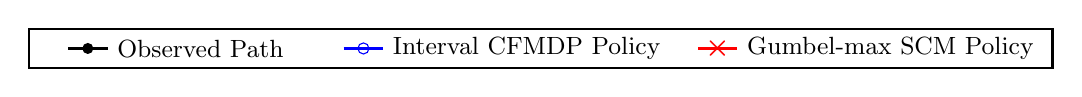
\begin{tikzpicture}[scale=1.0, every node/.style={scale=1.0}]
            \draw[thick, black] (-3, -0.25) rectangle (10, 0.25);
            %
            \draw[black, line width=1pt] (-2.5, 0.0) -- (-2,0.0);
            \fill[black] (-2.25,0.0) circle (2pt); %
            \node[right] at (-2,0.0) {\small Observed Path};
            
            %
            \draw[blue, line width=1pt] (1.0,0.0) -- (1.5,0.0);
            \node[draw=blue, circle, minimum size=4pt, inner sep=0pt] at (1.25,0.0) {}; %
            \node[right] at (1.5,0.0) {\small Interval CFMDP Policy};
            
            %
            \draw[red, line width=1pt] (5.5,0) -- (6,0);
            \node[red] at (5.75,0) {$\boldsymbol{\times}$}; %
            \node[right] at (6,0) {\small Gumbel-max SCM Policy};
        \end{tikzpicture}
    }\\
    %
    \subfigure[\footnotesize Lowest cumulative reward: Interval CFMDP ($312$), Gumbel-max SCM ($312$)]{%
        \resizebox{0.76\columnwidth}{!}{
             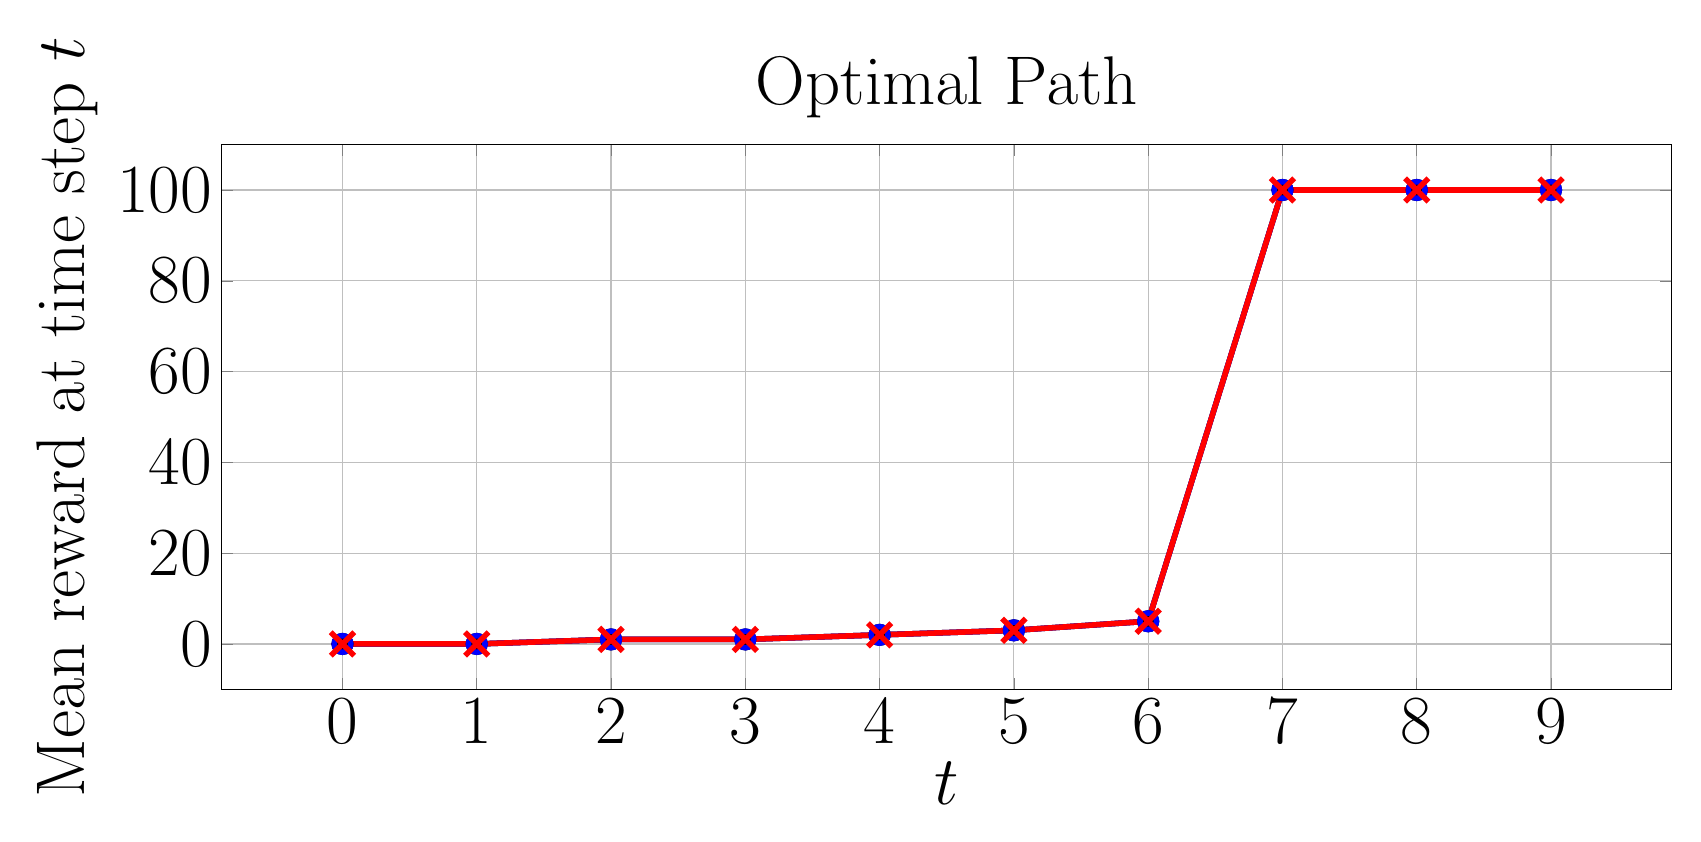
\begin{tikzpicture}
                \begin{axis}[
                    xlabel={$t$},
                    ylabel={Mean reward at time step $t$},
                    title={Optimal Path},
                    grid=both,
                    width=20cm, height=8.5cm,
                    every axis/.style={font=\Huge},
                    %
                ]
                \addplot[
                    color=black, %
                    mark=*, %
                    line width=2pt,
                    mark size=3pt,
                    error bars/.cd,
                    y dir=both, %
                    y explicit, %
                    error bar style={line width=1pt,solid},
                    error mark options={line width=1pt,mark size=4pt,rotate=90}
                ]
                coordinates {
                    (0, 0.0)  +- (0, 0.0)
                    (1, 0.0)  +- (0, 0.0) 
                    (2, 1.0)  +- (0, 0.0) 
                    (3, 1.0)  +- (0, 0.0)
                    (4, 2.0)  +- (0, 0.0)
                    (5, 3.0) +- (0, 0.0)
                    (6, 5.0) +- (0, 0.0)
                    (7, 100.0) +- (0, 0.0)
                    (8, 100.0) +- (0, 0.0)
                    (9, 100.0) +- (0, 0.0)
                };
                %
                \addplot[
                    color=blue, %
                    mark=o, %
                    line width=2pt,
                    mark size=3pt,
                    error bars/.cd,
                    y dir=both, %
                    y explicit, %
                    error bar style={line width=1pt,solid},
                    error mark options={line width=1pt,mark size=4pt,rotate=90}
                ]
                 coordinates {
                    (0, 0.0)  +- (0, 0.0)
                    (1, 0.0)  +- (0, 0.0) 
                    (2, 1.0)  +- (0, 0.0) 
                    (3, 1.0)  +- (0, 0.0)
                    (4, 2.0)  +- (0, 0.0)
                    (5, 3.0) +- (0, 0.0)
                    (6, 5.0) +- (0, 0.0)
                    (7, 100.0) +- (0, 0.0)
                    (8, 100.0) +- (0, 0.0)
                    (9, 100.0) +- (0, 0.0)
                };
                %
                \addplot[
                    color=red, %
                    mark=x, %
                    line width=2pt,
                    mark size=6pt,
                    error bars/.cd,
                    y dir=both, %
                    y explicit, %
                    error bar style={line width=1pt,solid},
                    error mark options={line width=1pt,mark size=4pt,rotate=90}
                ]
                coordinates {
                    (0, 0.0)  +- (0, 0.0)
                    (1, 0.0)  +- (0, 0.0) 
                    (2, 1.0)  +- (0, 0.0) 
                    (3, 1.0)  +- (0, 0.0)
                    (4, 2.0)  +- (0, 0.0)
                    (5, 3.0) +- (0, 0.0)
                    (6, 5.0) +- (0, 0.0)
                    (7, 100.0) +- (0, 0.0)
                    (8, 100.0) +- (0, 0.0)
                    (9, 100.0) +- (0, 0.0)
                };
                \end{axis}
            \end{tikzpicture}
         }
    }
    \hspace{1cm}
    \subfigure[\footnotesize Lowest cumulative reward: Interval CFMDP ($19$), Gumbel-max SCM ($-88$)]{%
         \resizebox{0.76\columnwidth}{!}{
            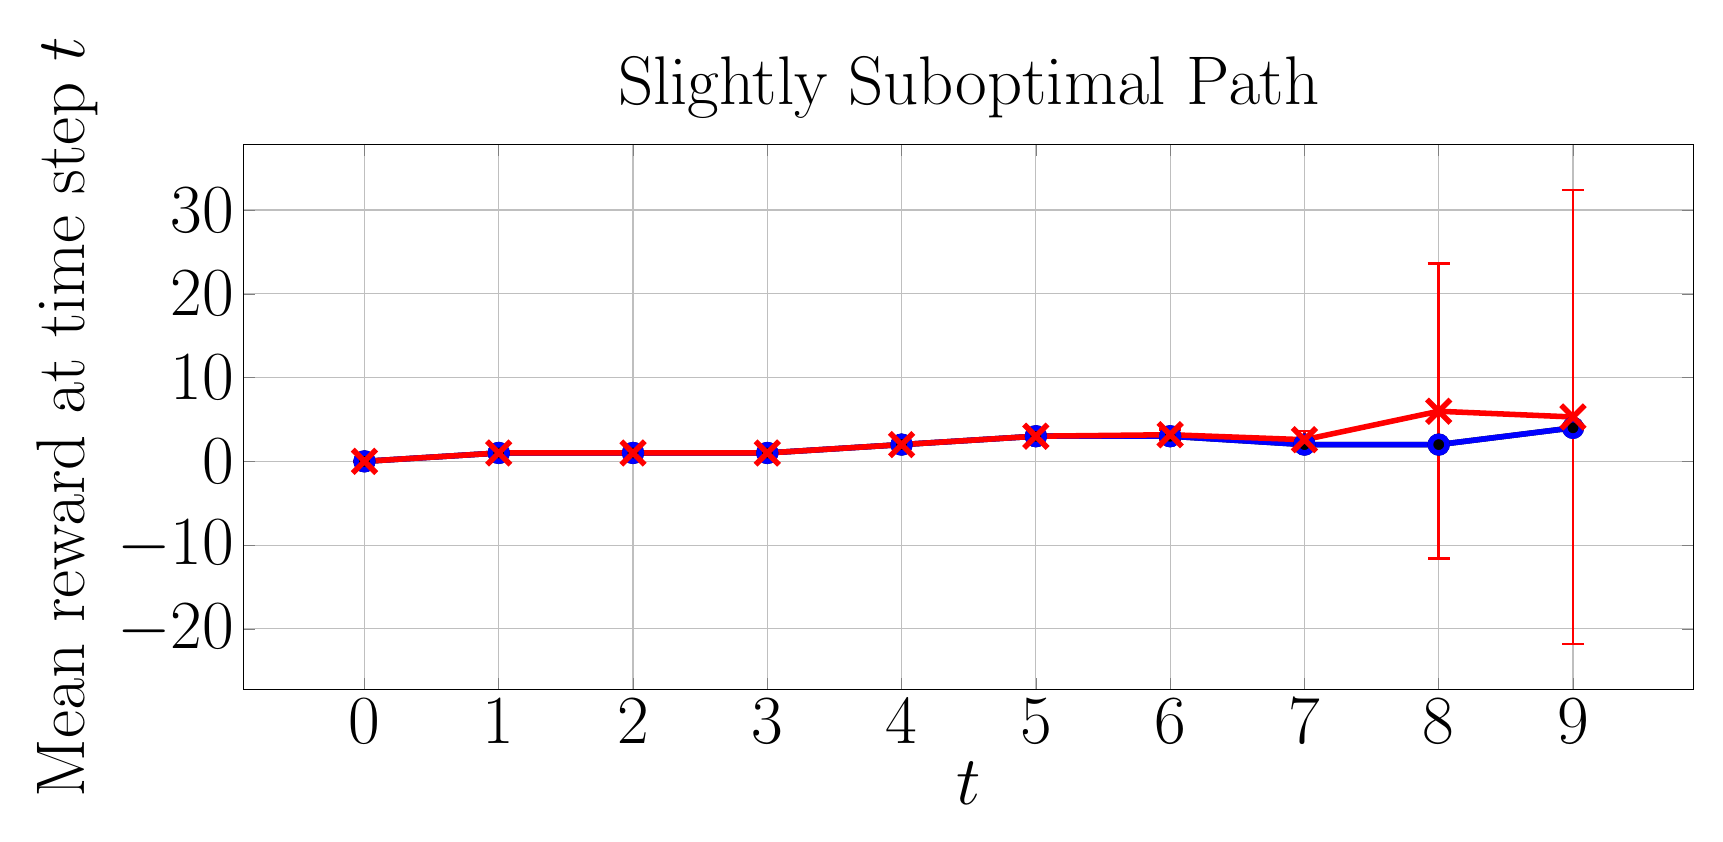
\begin{tikzpicture}
                \begin{axis}[
                    xlabel={$t$},
                    ylabel={Mean reward at time step $t$},
                    title={Slightly Suboptimal Path},
                    grid=both,
                    width=20cm, height=8.5cm,
                    every axis/.style={font=\Huge},
                    %
                ]
                \addplot[
                    color=black, %
                    mark=*, %
                    line width=2pt,
                    mark size=3pt,
                    error bars/.cd,
                    y dir=both, %
                    y explicit, %
                    error bar style={line width=1pt,solid},
                    error mark options={line width=1pt,mark size=4pt,rotate=90}
                ]
              coordinates {
                    (0, 0.0)  +- (0, 0.0)
                    (1, 1.0)  +- (0, 0.0) 
                    (2, 1.0)  +- (0, 0.0) 
                    (3, 1.0)  +- (0, 0.0)
                    (4, 2.0)  +- (0, 0.0)
                    (5, 3.0) +- (0, 0.0)
                    (6, 3.0) +- (0, 0.0)
                    (7, 2.0) +- (0, 0.0)
                    (8, 2.0) +- (0, 0.0)
                    (9, 4.0) +- (0, 0.0)
                };
                %
                \addplot[
                    color=blue, %
                    mark=o, %
                    line width=2pt,
                    mark size=3pt,
                    error bars/.cd,
                    y dir=both, %
                    y explicit, %
                    error bar style={line width=1pt,solid},
                    error mark options={line width=1pt,mark size=4pt,rotate=90}
                ]
              coordinates {
                    (0, 0.0)  +- (0, 0.0)
                    (1, 1.0)  +- (0, 0.0) 
                    (2, 1.0)  +- (0, 0.0) 
                    (3, 1.0)  +- (0, 0.0)
                    (4, 2.0)  +- (0, 0.0)
                    (5, 3.0) +- (0, 0.0)
                    (6, 3.0) +- (0, 0.0)
                    (7, 2.0) +- (0, 0.0)
                    (8, 2.0) +- (0, 0.0)
                    (9, 4.0) +- (0, 0.0)
                };
                %
                \addplot[
                    color=red, %
                    mark=x, %
                    line width=2pt,
                    mark size=6pt,
                    error bars/.cd,
                    y dir=both, %
                    y explicit, %
                    error bar style={line width=1pt,solid},
                    error mark options={line width=1pt,mark size=4pt,rotate=90}
                ]
                coordinates {
                    (0, 0.0)  +- (0, 0.0)
                    (1, 1.0)  +- (0, 0.0) 
                    (2, 1.0)  +- (0, 0.0) 
                    (3, 1.0)  +- (0, 0.0)
                    (4, 2.0)  += (0, 0.0)
                    (5, 3.0)  += (0, 0.0)
                    (6, 3.17847) += (0, 0.62606746) -= (0, 0.62606746)
                    (7, 2.5832885) += (0, 1.04598233) -= (0, 1.04598233)
                    (8, 5.978909) += (0, 17.60137623) -= (0, 17.60137623)
                    (9, 5.297059) += (0, 27.09227512) -= (0, 27.09227512)
                };
                \end{axis}
            \end{tikzpicture}
         }
    }\\[-1.5pt]
    \subfigure[\footnotesize Lowest cumulative reward: Interval CFMDP ($14$), Gumbel-max SCM ($-598$)]{%
         \resizebox{0.76\columnwidth}{!}{
             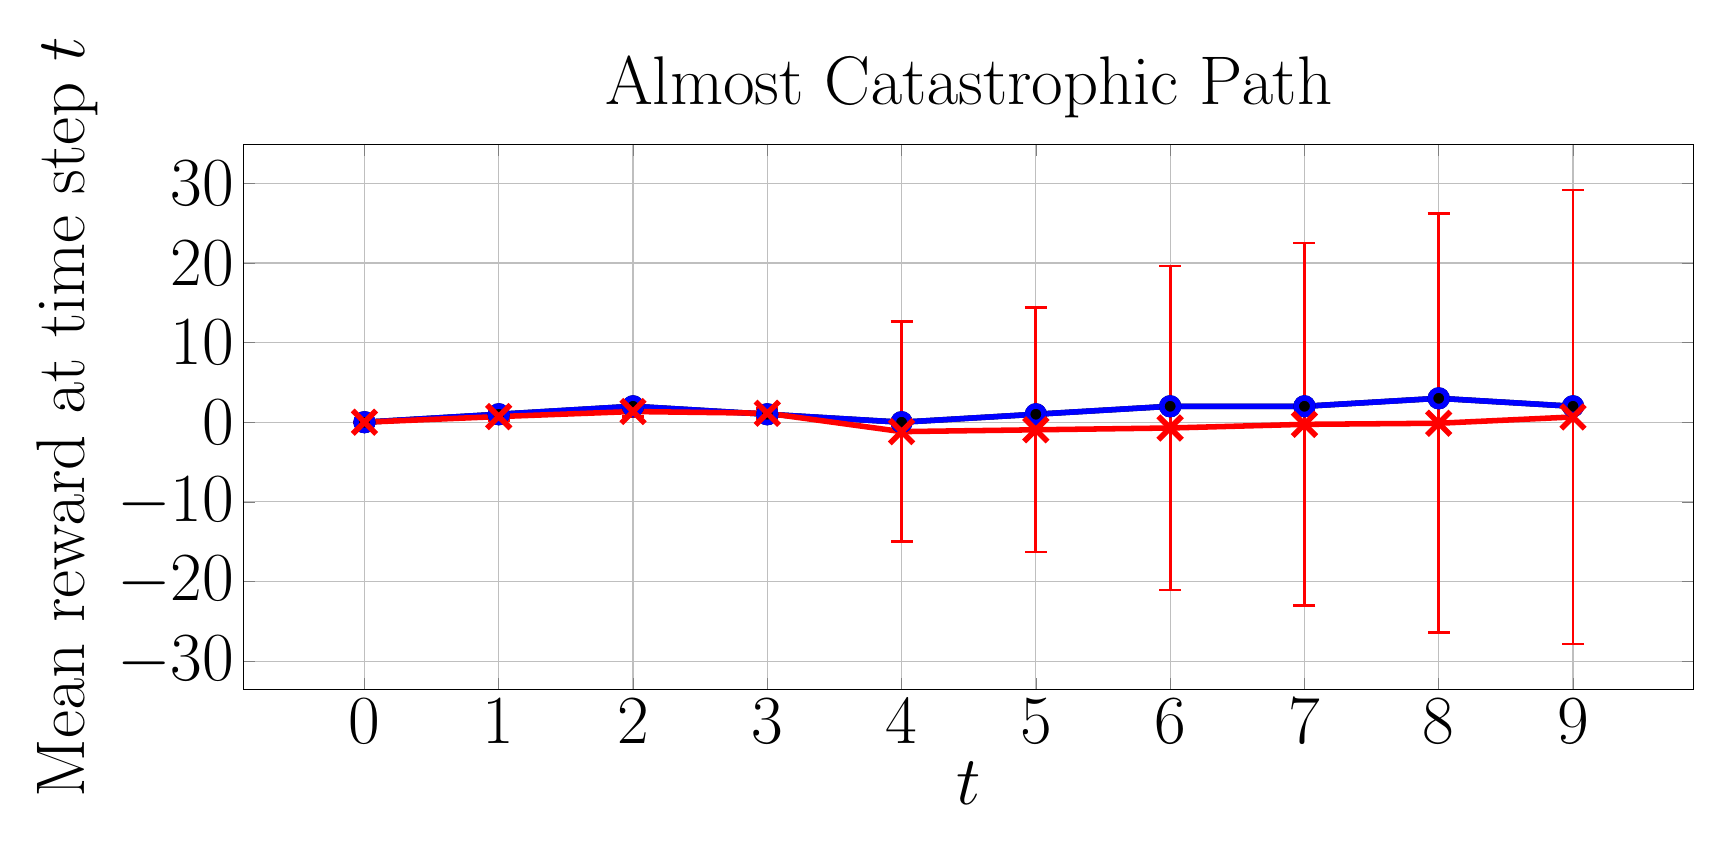
\begin{tikzpicture}
                \begin{axis}[
                    xlabel={$t$},
                    ylabel={Mean reward at time step $t$},
                    title={Almost Catastrophic Path},
                    grid=both,
                    width=20cm, height=8.5cm,
                    every axis/.style={font=\Huge},
                    %
                ]
                \addplot[
                    color=black, %
                    mark=*, %
                    line width=2pt,
                    mark size=3pt,
                    error bars/.cd,
                    y dir=both, %
                    y explicit, %
                    error bar style={line width=1pt,solid},
                    error mark options={line width=1pt,mark size=4pt,rotate=90}
                ]
                coordinates {
                    (0, 0.0)  +- (0, 0.0)
                    (1, 1.0)  +- (0, 0.0) 
                    (2, 2.0)  +- (0, 0.0) 
                    (3, 1.0)  +- (0, 0.0)
                    (4, 0.0)  +- (0, 0.0)
                    (5, 1.0) +- (0, 0.0)
                    (6, 2.0) +- (0, 0.0)
                    (7, 2.0) +- (0, 0.0)
                    (8, 3.0) +- (0, 0.0)
                    (9, 2.0) +- (0, 0.0)
                };
                %
                \addplot[
                    color=blue, %
                    mark=o, %
                    line width=2pt,
                    mark size=3pt,
                    error bars/.cd,
                    y dir=both, %
                    y explicit, %
                    error bar style={line width=1pt,solid},
                    error mark options={line width=1pt,mark size=4pt,rotate=90}
                ]
                coordinates {
                    (0, 0.0)  +- (0, 0.0)
                    (1, 1.0)  +- (0, 0.0) 
                    (2, 2.0)  +- (0, 0.0) 
                    (3, 1.0)  +- (0, 0.0)
                    (4, 0.0)  +- (0, 0.0)
                    (5, 1.0) +- (0, 0.0)
                    (6, 2.0) +- (0, 0.0)
                    (7, 2.0) +- (0, 0.0)
                    (8, 3.0) +- (0, 0.0)
                    (9, 2.0) +- (0, 0.0)
                };
                %
                \addplot[
                    color=red, %
                    mark=x, %
                    line width=2pt,
                    mark size=6pt,
                    error bars/.cd,
                    y dir=both, %
                    y explicit, %
                    error bar style={line width=1pt,solid},
                    error mark options={line width=1pt,mark size=4pt,rotate=90}
                ]
                coordinates {
                    (0, 0.0)  +- (0, 0.0)
                    (1, 0.7065655)  +- (0, 0.4553358) 
                    (2, 1.341673)  +- (0, 0.67091621) 
                    (3, 1.122926)  +- (0, 0.61281824)
                    (4, -1.1821935)  +- (0, 13.82444042)
                    (5, -0.952399)  +- (0, 15.35195457)
                    (6, -0.72672) +- (0, 20.33508414)
                    (7, -0.268983) +- (0, 22.77861454)
                    (8, -0.1310835) +- (0, 26.31013314)
                    (9, 0.65806) +- (0, 28.50670214)
                };
                %
            %
            %
            %
            %
            %
            %
            %
            %
            %
            %
            %
            %
            %
            %
            %
            %
            %
            %
                \end{axis}
            \end{tikzpicture}
         }
    }
    \hspace{1cm}
    \subfigure[\footnotesize Lowest cumulative reward: Interval CFMDP ($-698$), Gumbel-max SCM ($-698$)]{%
         \resizebox{0.76\columnwidth}{!}{
            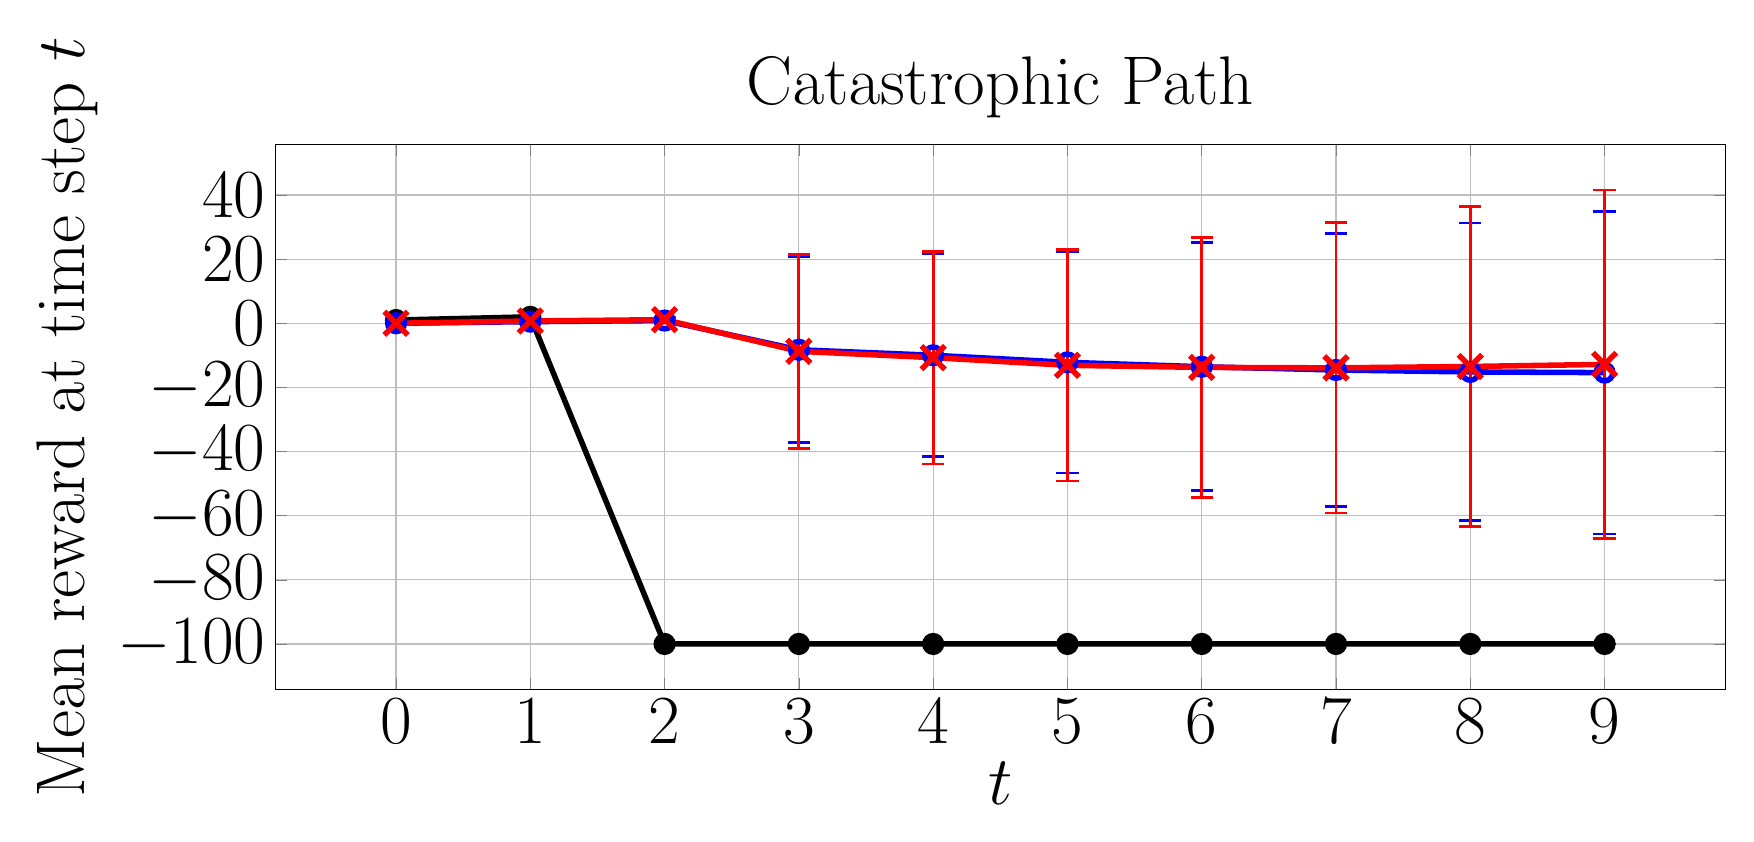
\begin{tikzpicture}
                \begin{axis}[
                    xlabel={$t$},
                    ylabel={Mean reward at time step $t$},
                    title={Catastrophic Path},
                    grid=both,
                    width=20cm, height=8.5cm,
                    every axis/.style={font=\Huge},
                    %
                ]
                \addplot[
                    color=black, %
                    mark=*, %
                    line width=2pt,
                    mark size=3pt,
                    error bars/.cd,
                    y dir=both, %
                    y explicit, %
                    error bar style={line width=1pt,solid},
                    error mark options={line width=1pt,mark size=4pt,rotate=90}
                ]
                coordinates {
                    (0, 1.0)  +- (0, 0.0)
                    (1, 2.0)  +- (0, 0.0) 
                    (2, -100.0)  +- (0, 0.0) 
                    (3, -100.0)  +- (0, 0.0)
                    (4, -100.0)  +- (0, 0.0)
                    (5, -100.0) +- (0, 0.0)
                    (6, -100.0) +- (0, 0.0)
                    (7, -100.0) +- (0, 0.0)
                    (8, -100.0) +- (0, 0.0)
                    (9, -100.0) +- (0, 0.0)
                };
                %
                \addplot[
                    color=blue, %
                    mark=o, %
                    line width=2pt,
                    mark size=3pt,
                    error bars/.cd,
                    y dir=both, %
                    y explicit, %
                    error bar style={line width=1pt,solid},
                    error mark options={line width=1pt,mark size=4pt,rotate=90}
                ]
                coordinates {
                    (0, 0.0)  +- (0, 0.0)
                    (1, 0.504814)  +- (0, 0.49997682) 
                    (2, 0.8439835)  +- (0, 0.76831917) 
                    (3, -8.2709165)  +- (0, 28.93656754)
                    (4, -9.981082)  +- (0, 31.66825363)
                    (5, -12.1776325) +- (0, 34.53463233)
                    (6, -13.556076) +- (0, 38.62845372)
                    (7, -14.574418) +- (0, 42.49603359)
                    (8, -15.1757075) +- (0, 46.41913968)
                    (9, -15.3900395) +- (0, 50.33563368)
                };
                %
                \addplot[
                    color=red, %
                    mark=x, %
                    line width=2pt,
                    mark size=6pt,
                    error bars/.cd,
                    y dir=both, %
                    y explicit, %
                    error bar style={line width=1pt,solid},
                    error mark options={line width=1pt,mark size=4pt,rotate=90}
                ]
                coordinates {
                    (0, 0.0)  +- (0, 0.0)
                    (1, 0.701873)  +- (0, 0.45743556) 
                    (2, 1.1227805)  +- (0, 0.73433129) 
                    (3, -8.7503255)  +- (0, 30.30257976)
                    (4, -10.722092)  +- (0, 33.17618589)
                    (5, -13.10721)  +- (0, 36.0648089)
                    (6, -13.7631645) +- (0, 40.56553451)
                    (7, -13.909043) +- (0, 45.23829402)
                    (8, -13.472517) +- (0, 49.96270296)
                    (9, -12.8278835) +- (0, 54.38618735)
                };
                %
            %
            %
            %
            %
            %
            %
            %
            %
            %
            %
            %
            %
            %
            %
            %
            %
            %
            %
                \end{axis}
            \end{tikzpicture}
         }
    }
    \caption{Average instant reward of CF paths induced by policies on GridWorld $p=0.4$.}
    \label{fig: reward p=0.4}
\end{figure*}

\subsection{Experimental Setup}
To compare policy performance, we measure the average rewards of counterfactual paths induced by our policy and the Gumbel-max policy by uniformly sampling $200$ counterfactual MDPs from the ICFMDP and generating $10,000$ counterfactual paths over each sampled CFMDP. \jl{Since the interval CFMDP depends on the observed path, we select $4$  paths of varying optimality to evaluate how the observed path impacts the performance of both policies: an optimal path, a slightly suboptimal path that could reach the optimal reward with a few changes, a catastrophic path that enters a catastrophic, terminal state with low reward, and an almost catastrophic path that was close to entering a catastrophic state.} When measuring the average probability bound widths and execution time needed to generate the ICFMDPs, we averaged over $20$ randomly generated observed paths
\footnote{Further training details are provided in Appendix \ref{app: training details}, and the code is provided at \href{https://github.com/ddv-lab/robust-cf-inference-in-MDPs}{https://github.com/ddv-lab/robust-cf-inference-in-MDPs}
%
%
.}.

\subsection{GridWorld}
\jl{The GridWorld MDP is a $4 \times 4$ grid where an agent must navigate from the top-left corner to the goal state in the bottom-right corner, avoiding a dangerous terminal state in the centre. At each time step, the agent can move up, down, left, or right, but there is a small probability (controlled by hyper-parameter $p$) of moving in an unintended direction. As the agent nears the goal, the reward for each state increases, culminating in a reward of $+100$ for reaching the goal. Entering the dangerous state results in a penalty of $-100$. We use two versions of GridWorld: a less stochastic version with $p=0.9$ (i.e., $90$\% chance of moving in the chosen direction) and a more stochastic version with $p=0.4$.}

\paragraph{GridWorld ($p=0.9$)}
When $p=0.9$, the counterfactual probability bounds are typically narrow (see Table \ref{tab:nonzero_probs} for average measurements). Consequently, as shown in Figure \ref{fig: reward p=0.9}, both policies are nearly identical and perform similarly well across the optimal, slightly suboptimal, and catastrophic paths.
%
However, for the almost catastrophic path, the interval CFMDP path is more conservative and follows the observed path more closely (as this is where the probability bounds are narrowest), which typically requires one additional step to reach the goal state than the Gumbel-max SCM policy.
%

\paragraph{GridWorld ($p=0.4$)}
\jl{When $p=0.4$, the GridWorld environment becomes more uncertain, increasing the risk of entering the dangerous state even if correct actions are chosen. Thus, as shown in Figure \ref{fig: reward p=0.4}, the interval CFMDP policy adopts a more conservative approach, avoiding deviation from the observed policy if it cannot guarantee higher counterfactual rewards (see the slightly suboptimal and almost catastrophic paths), whereas the Gumbel-max SCM is inconsistent: it can yield higher rewards, but also much lower rewards, reflected in the wide error bars.} For the catastrophic path, both policies must deviate from the observed path to achieve a higher reward and, in this case, perform similarly.
%
%
%
%
\subsection{Sepsis}
The Sepsis MDP \citep{oberst2019counterfactual} simulates trajectories of Sepsis patients. Each state consists of four vital signs (heart rate, blood pressure, oxygen concentration, and glucose levels), categorised as low, normal, or high.
and three treatments that can be toggled on/off at each time step (8 actions in total). Unlike \citet{oberst2019counterfactual}, we scale rewards based on the number of out-of-range vital signs, between $-1000$ (patient dies) and $1000$ (patient discharged). \jl{Like the GridWorld $p=0.4$ experiment, the Sepsis MDP is highly uncertain, as many states are equally likely to lead to optimal and poor outcomes. Thus, as shown in Figure \ref{fig: reward sepsis}, both policies follow the observed optimal and almost catastrophic paths to guarantee rewards are no worse than the observation.} However, improving the catastrophic path requires deviating from the observation. Here, the Gumbel-max SCM policy, on average, performs better than the interval CFMDP policy. But, since both policies have lower bounds clipped at $-1000$, neither policy reliably improves over the observation. In contrast, for the slightly suboptimal path, the interval CFMDP policy performs significantly better, shown by its higher lower bounds. 
Moreover, in these two cases, the worst-case counterfactual path generated by the interval CFMDP policy is better than that of the Gumbel-max SCM policy,
indicating its greater robustness.
%
\begin{figure*}
    \centering
     \resizebox{0.6\textwidth}{!}{
        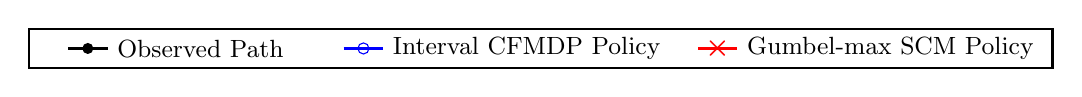
\begin{tikzpicture}[scale=1.0, every node/.style={scale=1.0}]
            \draw[thick, black] (-3, -0.25) rectangle (10, 0.25);
            %
            \draw[black, line width=1pt] (-2.5, 0.0) -- (-2,0.0);
            \fill[black] (-2.25,0.0) circle (2pt); %
            \node[right] at (-2,0.0) {\small Observed Path};
            
            %
            \draw[blue, line width=1pt] (1.0,0.0) -- (1.5,0.0);
            \node[draw=blue, circle, minimum size=4pt, inner sep=0pt] at (1.25,0.0) {}; %
            \node[right] at (1.5,0.0) {\small Interval CFMDP Policy};
            
            %
            \draw[red, line width=1pt] (5.5,0) -- (6,0);
            \node[red] at (5.75,0) {$\boldsymbol{\times}$}; %
            \node[right] at (6,0) {\small Gumbel-max SCM Policy};
        \end{tikzpicture}
    }\\
    \subfigure[\footnotesize Lowest cumulative reward: Interval CFMDP ($8000$), Gumbel-max SCM ($8000$)]{%
         \resizebox{0.76\columnwidth}{!}{
             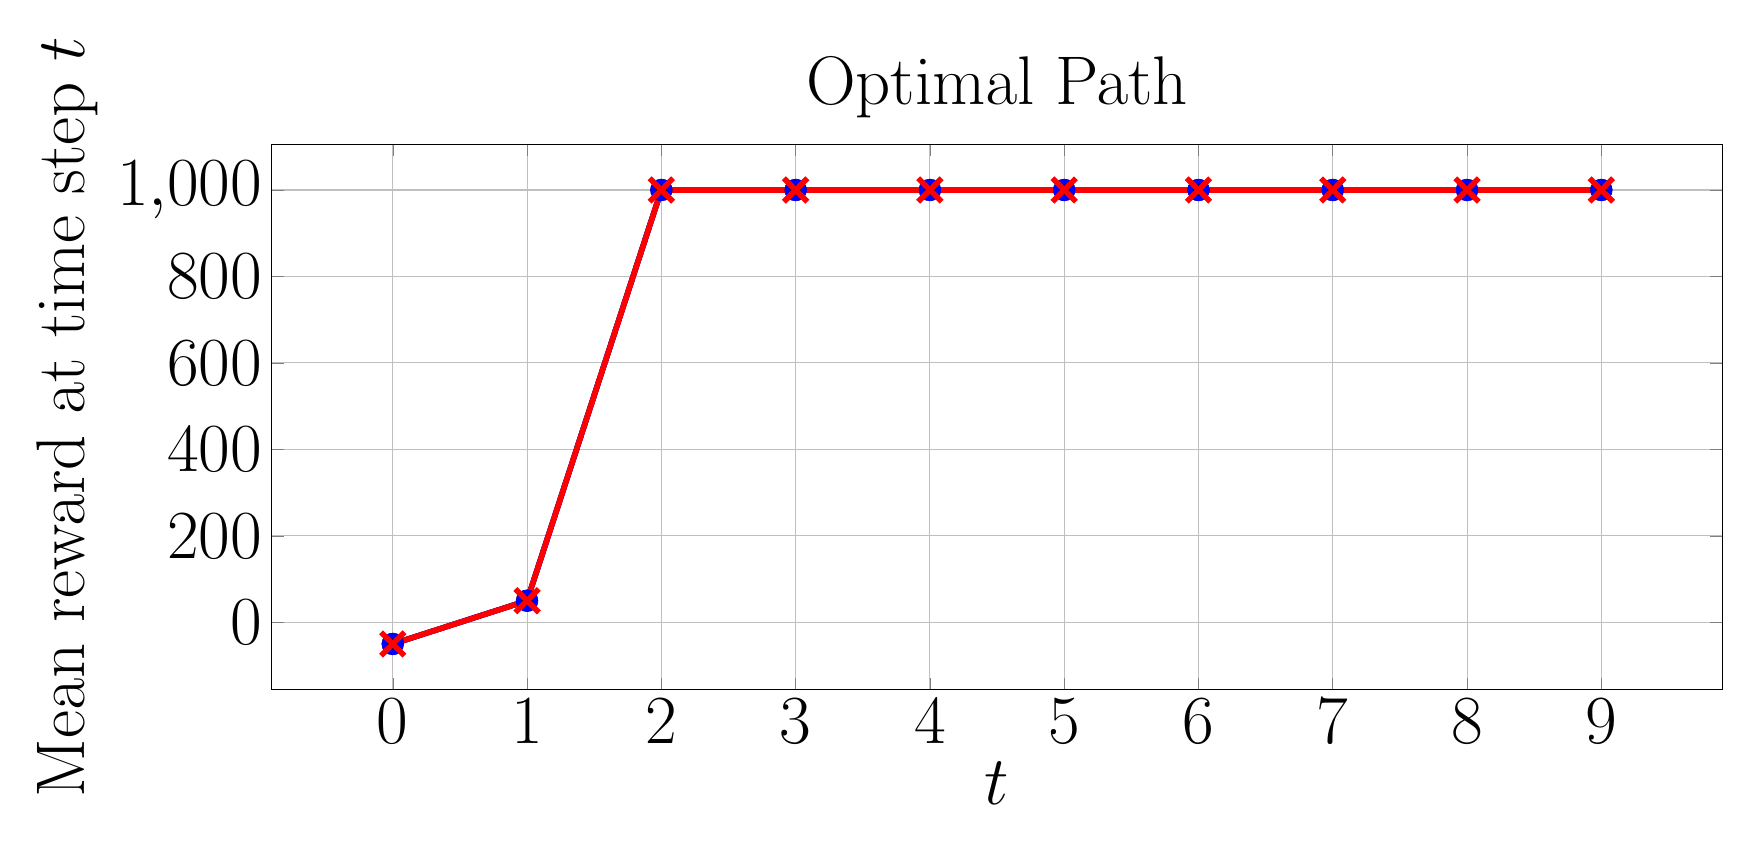
\begin{tikzpicture}
                \begin{axis}[
                    xlabel={$t$},
                    ylabel={Mean reward at time step $t$},
                    title={Optimal Path},
                    grid=both,
                    width=20cm, height=8.5cm,
                    every axis/.style={font=\Huge},
                    %
                ]
                \addplot[
                    color=black, %
                    mark=*, %
                    line width=2pt,
                    mark size=3pt,
                ]
                coordinates {
                    (0, -50.0)
                    (1, 50.0)
                    (2, 1000.0)
                    (3, 1000.0)
                    (4, 1000.0)
                    (5, 1000.0)
                    (6, 1000.0)
                    (7, 1000.0)
                    (8, 1000.0)
                    (9, 1000.0)
                };
                %
                \addplot[
                    color=blue, %
                    mark=o, %
                    line width=2pt,
                    mark size=3pt,
                    error bars/.cd,
                    y dir=both, %
                    y explicit, %
                    error bar style={line width=1pt,solid},
                    error mark options={line width=1pt,mark size=4pt,rotate=90}
                ]
                coordinates {
                    (0, -50.0)  +- (0, 0.0)
                    (1, 50.0)  +- (0, 0.0) 
                    (2, 1000.0)  +- (0, 0.0) 
                    (3, 1000.0)  +- (0, 0.0)
                    (4, 1000.0)  +- (0, 0.0)
                    (5, 1000.0) +- (0, 0.0)
                    (6, 1000.0) +- (0, 0.0)
                    (7, 1000.0) +- (0, 0.0)
                    (8, 1000.0) +- (0, 0.0)
                    (9, 1000.0) +- (0, 0.0)
                };
                %
                \addplot[
                    color=red, %
                    mark=x, %
                    line width=2pt,
                    mark size=6pt,
                    error bars/.cd,
                    y dir=both, %
                    y explicit, %
                    error bar style={line width=1pt,solid},
                    error mark options={line width=1pt,mark size=4pt,rotate=90}
                ]
                coordinates {
                    (0, -50.0)  +- (0, 0.0)
                    (1, 50.0)  +- (0, 0.0) 
                    (2, 1000.0)  +- (0, 0.0) 
                    (3, 1000.0)  +- (0, 0.0)
                    (4, 1000.0)  +- (0, 0.0)
                    (5, 1000.0) +- (0, 0.0)
                    (6, 1000.0) +- (0, 0.0)
                    (7, 1000.0) +- (0, 0.0)
                    (8, 1000.0) +- (0, 0.0)
                    (9, 1000.0) +- (0, 0.0)
                };
                %
                \end{axis}
            \end{tikzpicture}
         }
    }
    \hspace{1cm}
    \subfigure[\footnotesize Lowest cumulative reward: Interval CFMDP ($-5980$), Gumbel-max SCM ($-8000$)]{%
         \resizebox{0.76\columnwidth}{!}{
            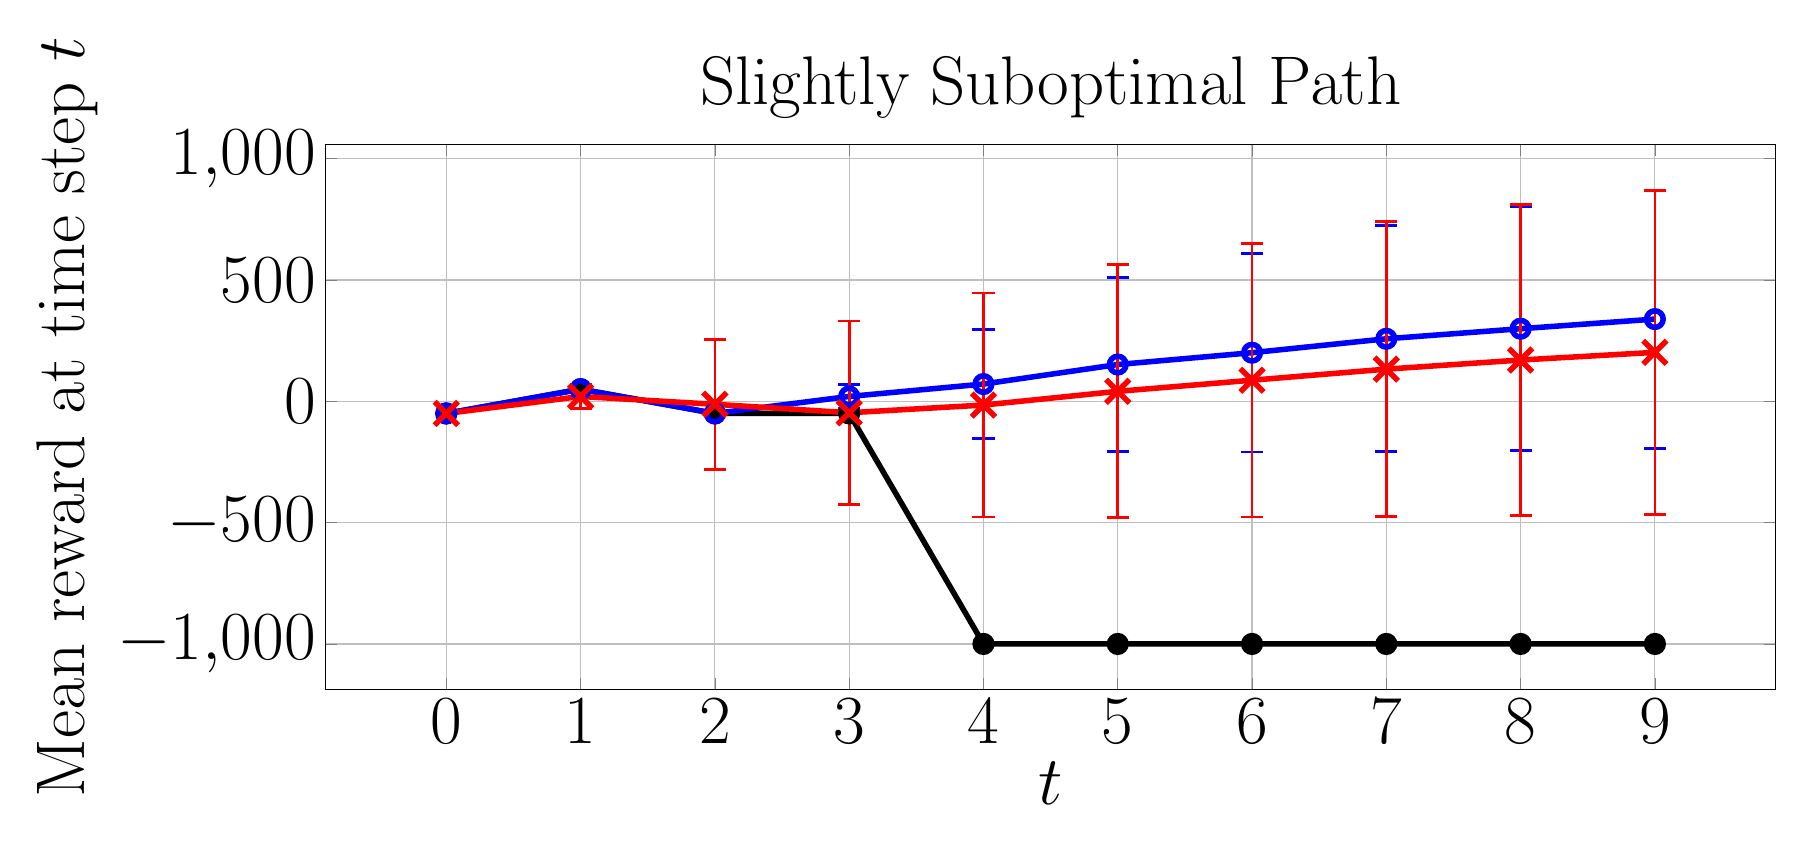
\begin{tikzpicture}
                \begin{axis}[
                    xlabel={$t$},
                    ylabel={Mean reward at time step $t$},
                    title={Slightly Suboptimal Path},
                    grid=both,
                    width=20cm, height=8.5cm,
                    every axis/.style={font=\Huge},
                    %
                ]
               \addplot[
                    color=black, %
                    mark=*, %
                    line width=2pt,
                    mark size=3pt,
                ]
                coordinates {
                    (0, -50.0)
                    (1, 50.0)
                    (2, -50.0)
                    (3, -50.0)
                    (4, -1000.0)
                    (5, -1000.0)
                    (6, -1000.0)
                    (7, -1000.0)
                    (8, -1000.0)
                    (9, -1000.0)
                };
                %
                \addplot[
                    color=blue, %
                    mark=o, %
                    line width=2pt,
                    mark size=3pt,
                    error bars/.cd,
                    y dir=both, %
                    y explicit, %
                    error bar style={line width=1pt,solid},
                    error mark options={line width=1pt,mark size=4pt,rotate=90}
                ]
                coordinates {
                    (0, -50.0)  +- (0, 0.0)
                    (1, 50.0)  +- (0, 0.0) 
                    (2, -50.0)  +- (0, 0.0) 
                    (3, 20.0631)  +- (0, 49.97539413)
                    (4, 71.206585)  +- (0, 226.02033693)
                    (5, 151.60797) +- (0, 359.23292559)
                    (6, 200.40593) +- (0, 408.86185176)
                    (7, 257.77948) +- (0, 466.10372804)
                    (8, 299.237465) +- (0, 501.82579506)
                    (9, 338.9129) +- (0, 532.06124996)
                };
                %
                \addplot[
                    color=red, %
                    mark=x, %
                    line width=2pt,
                    mark size=6pt,
                    error bars/.cd,
                    y dir=both, %
                    y explicit, %
                    error bar style={line width=1pt,solid},
                    error mark options={line width=1pt,mark size=4pt,rotate=90}
                ]
                coordinates {
                    (0, -50.0)  +- (0, 0.0)
                    (1, 20.00736)  +- (0, 49.99786741) 
                    (2, -12.282865)  +- (0, 267.598755) 
                    (3, -47.125995)  +- (0, 378.41755832)
                    (4, -15.381965)  +- (0, 461.77616558)
                    (5, 41.15459) +- (0, 521.53189262)
                    (6, 87.01595) +- (0, 564.22243126 )
                    (7, 132.62376) +- (0, 607.31338037)
                    (8, 170.168145) +- (0, 641.48013693)
                    (9, 201.813135) +- (0, 667.29441777)
                };
                %
                %
                %
                %
                %
                %
                %
                %
                %
                %
                %
                %
                %
                %
                %
                %
                %
                %
                %
                \end{axis}
            \end{tikzpicture}
         }
    }\\[-1.5pt]
    \subfigure[\footnotesize Lowest cumulative reward: Interval CFMDP ($100$), Gumbel-max SCM ($100$)]{%
         \resizebox{0.76\columnwidth}{!}{
             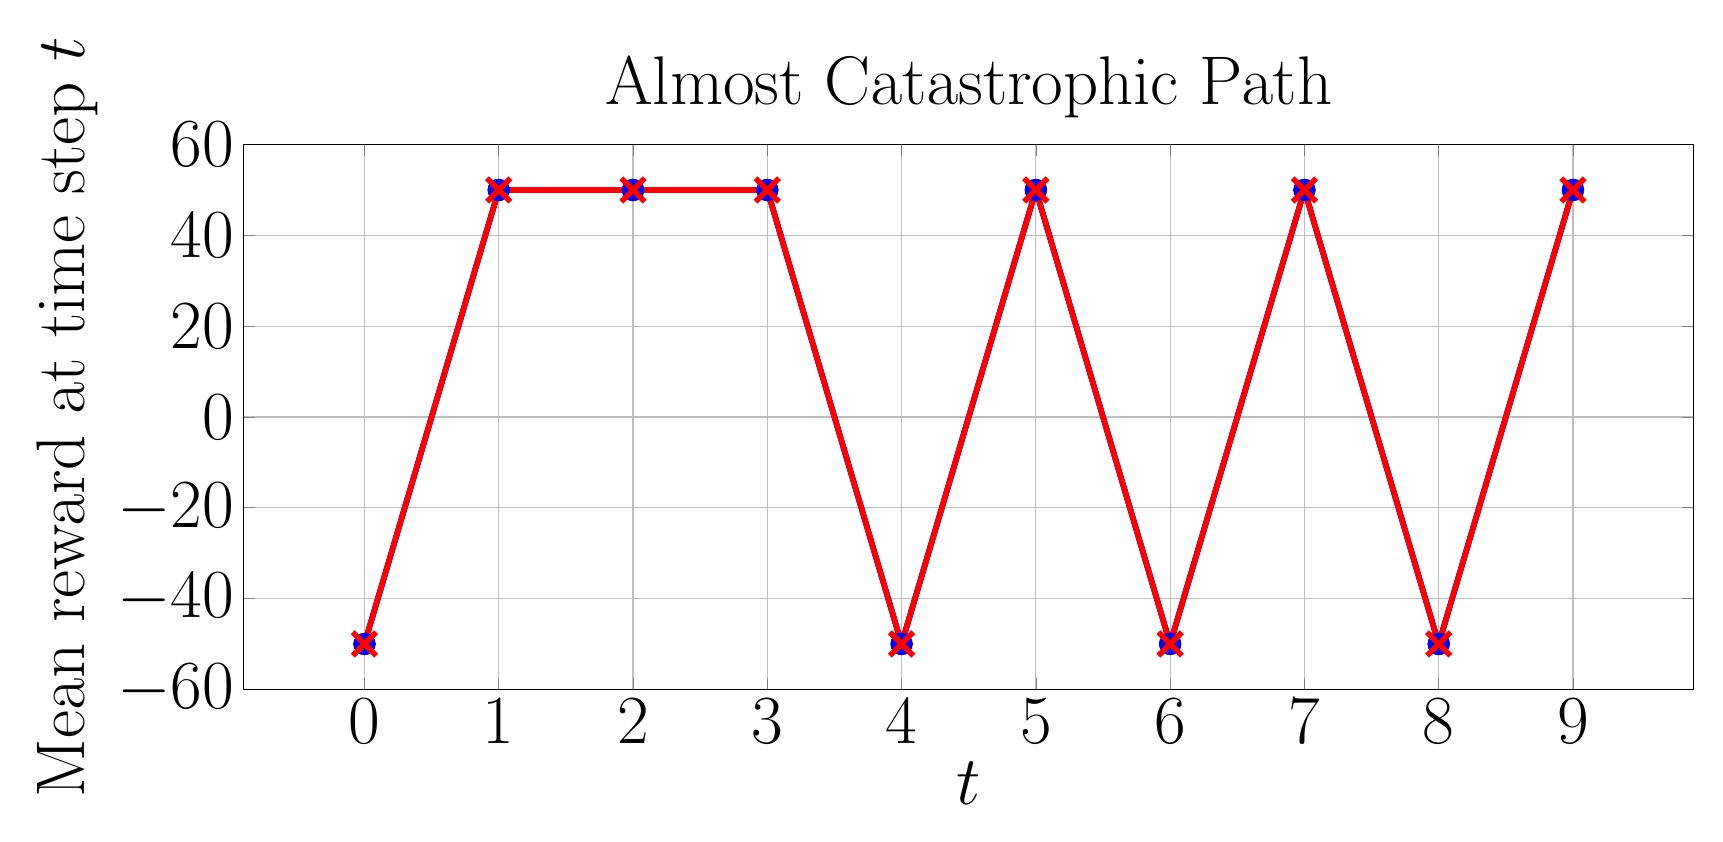
\begin{tikzpicture}
                \begin{axis}[
                    xlabel={$t$},
                    ylabel={Mean reward at time step $t$},
                    title={Almost Catastrophic Path},
                    grid=both,
                    every axis/.style={font=\Huge},
                    width=20cm, height=8.5cm,
                    %
                ]
               \addplot[
                    color=black, %
                    mark=*, %
                    line width=2pt,
                    mark size=3pt,
                ]
                coordinates {
                    (0, -50.0)
                    (1, 50.0)
                    (2, 50.0)
                    (3, 50.0)
                    (4, -50.0)
                    (5, 50.0)
                    (6, -50.0)
                    (7, 50.0)
                    (8, -50.0)
                    (9, 50.0)
                };
                %
                %
                \addplot[
                    color=blue, %
                    mark=o, %
                    line width=2pt,
                    mark size=3pt,
                    error bars/.cd,
                    y dir=both, %
                    y explicit, %
                    error bar style={line width=1pt,solid},
                    error mark options={line width=1pt,mark size=4pt,rotate=90}
                ]
                coordinates {
                    (0, -50.0)  +- (0, 0.0)
                    (1, 50.0)  +- (0, 0.0) 
                    (2, 50.0)  +- (0, 0.0) 
                    (3, 50.0)  +- (0, 0.0)
                    (4, -50.0)  +- (0, 0.0)
                    (5, 50.0) +- (0, 0.0)
                    (6, -50.0) +- (0, 0.0)
                    (7, 50.0) +- (0, 0.0)
                    (8, -50.0) +- (0, 0.0)
                    (9, 50.0) +- (0, 0.0)
                };
                %
                \addplot[
                    color=red, %
                    mark=x, %
                    line width=2pt,
                    mark size=6pt,
                    error bars/.cd,
                    y dir=both, %
                    y explicit, %
                    error bar style={line width=1pt,solid},
                    error mark options={line width=1pt,mark size=4pt,rotate=90}
                ]
                coordinates {
                    (0, -50.0)  +- (0, 0.0)
                    (1, 50.0)  +- (0, 0.0) 
                    (2, 50.0)  +- (0, 0.0) 
                    (3, 50.0)  +- (0, 0.0)
                    (4, -50.0)  +- (0, 0.0)
                    (5, 50.0) +- (0, 0.0)
                    (6, -50.0) +- (0, 0.0)
                    (7, 50.0) +- (0, 0.0)
                    (8, -50.0) +- (0, 0.0)
                    (9, 50.0) +- (0, 0.0)
                };
                %
                %
                %
                %
                %
                %
                %
                %
                %
                %
                %
                %
                %
                %
                %
                %
                %
                %
                %
                \end{axis}
            \end{tikzpicture}
         }
    }
    \hspace{1cm}
    \subfigure[\footnotesize Lowest cumulative reward: Interval CFMDP ($-7150$), Gumbel-max SCM ($-9050$)]{%
         \resizebox{0.76\columnwidth}{!}{
            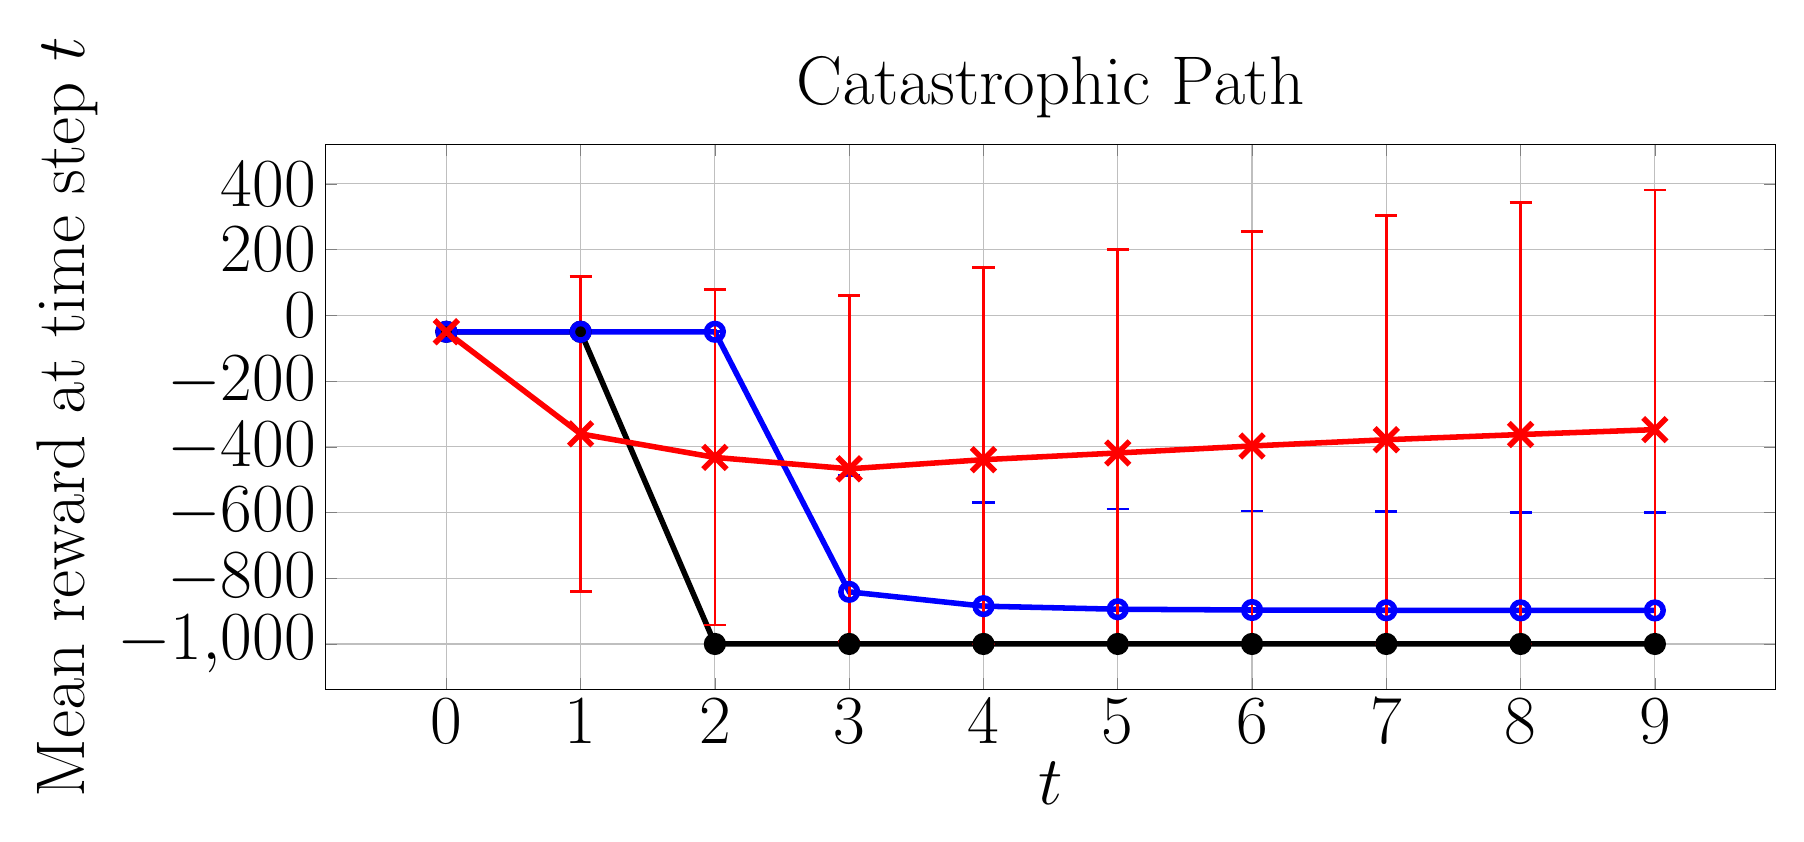
\begin{tikzpicture}
                \begin{axis}[
                    xlabel={$t$},
                    ylabel={Mean reward at time step $t$},
                    title={Catastrophic Path},
                    grid=both,
                    width=20cm, height=8.5cm,
                    every axis/.style={font=\Huge},
                    %
                ]
               \addplot[
                    color=black, %
                    mark=*, %
                    line width=2pt,
                    mark size=3pt,
                ]
                coordinates {
                    (0, -50.0)
                    (1, -50.0)
                    (2, -1000.0)
                    (3, -1000.0)
                    (4, -1000.0)
                    (5, -1000.0)
                    (6, -1000.0)
                    (7, -1000.0)
                    (8, -1000.0)
                    (9, -1000.0)
                };
                %
                %
                \addplot[
                    color=blue, %
                    mark=o, %
                    line width=2pt,
                    mark size=3pt,
                    error bars/.cd,
                    y dir=both, %
                    y explicit, %
                    error bar style={line width=1pt,solid},
                    error mark options={line width=1pt,mark size=4pt,rotate=90}
                ]
                coordinates {
                    (0, -50.0)  +- (0, 0.0)
                    (1, -50.0)  +- (0, 0.0) 
                    (2, -50.0)  +- (0, 0.0) 
                    (3, -841.440725)  += (0, 354.24605512) -= (0, 158.559275)
                    (4, -884.98225)  += (0, 315.37519669) -= (0, 115.01775)
                    (5, -894.330425) += (0, 304.88572805) -= (0, 105.669575)
                    (6, -896.696175) += (0, 301.19954514) -= (0, 103.303825)
                    (7, -897.4635) += (0, 299.61791279) -= (0, 102.5365)
                    (8, -897.77595) += (0, 298.80392585) -= (0, 102.22405)
                    (9, -897.942975) += (0, 298.32920557) -= (0, 102.057025)
                };
                %
                \addplot[
                    color=red, %
                    mark=x, %
                    line width=2pt,
                    mark size=6pt,
                    error bars/.cd,
                    y dir=both, %
                    y explicit, %
                    error bar style={line width=1pt,solid},
                    error mark options={line width=1pt,mark size=4pt,rotate=90}
                ]
            coordinates {
                    (0, -50.0)  +- (0, 0.0)
                    (1, -360.675265)  +- (0, 479.39812699) 
                    (2, -432.27629)  +- (0, 510.38620897) 
                    (3, -467.029545)  += (0, 526.36009628) -= (0, 526.36009628)
                    (4, -439.17429)  += (0, 583.96638919) -= (0, 560.82571)
                    (5, -418.82704) += (0, 618.43027478) -= (0, 581.17296)
                    (6, -397.464895) += (0, 652.67322574) -= (0, 602.535105)
                    (7, -378.49052) += (0, 682.85407033) -= (0, 621.50948)
                    (8, -362.654195) += (0, 707.01412023) -= (0, 637.345805)
                    (9, -347.737935) += (0, 729.29076479) -= (0, 652.262065)
                };
                %
                %
                %
                %
                %
                %
                %
                %
                %
                %
                %
                %
                %
                %
                %
                %
                %
                %
                %
                \end{axis}
            \end{tikzpicture}
         }
    }
    \caption{Average instant reward of CF paths induced by policies on Sepsis.}
    \label{fig: reward sepsis}
\end{figure*}

%
%
%
\subsection{Interval CFMDP Bounds}
%
%
Table \ref{tab:nonzero_probs} presents the mean counterfactual probability bound widths (excluding transitions where the upper bound is $0$) for each MDP, averaged over 20 observed paths. We compare the bounds under counterfactual stability (CS) and monotonicity (M) assumptions, CS alone, and no assumptions. This shows that the assumptions marginally reduce the bound widths, indicating the assumptions tighten the bounds without excluding too many causal models, as intended.
\renewcommand{\arraystretch}{1}

\begin{table}
\centering
\caption{Mean width of counterfactual probability bounds}
\resizebox{0.8\columnwidth}{!}{%
\begin{tabular}{|c|c|c|c|}
\hline
\multirow{2}{*}{\textbf{Environment}} & \multicolumn{3}{c|}{\textbf{Assumptions}} \\ \cline{2-4}
 & \textbf{CS + M} & \textbf{CS} & \textbf{None\tablefootnote{\jl{Equivalent to \citet{li2024probabilities}'s bounds (see Section \ref{sec: equivalence with Li}).}}} \\ \hline
\textbf{GridWorld} ($p=0.9$) & 0.0817 & 0.0977 & 0.100 \\ \hline
\textbf{GridWorld} ($p=0.4$) & 0.552  & 0.638  & 0.646 \\ \hline
\textbf{Sepsis} & 0.138 & 0.140 & 0.140 \\ \hline
\end{tabular}
}
\label{tab:nonzero_probs}
\end{table}


\subsection{Execution Times}
Table \ref{tab: times} compares the average time needed to generate the interval CFMDP vs.\ the Gumbel-max SCM CFMDP for 20 observations.
The GridWorld algorithms were run single-threaded, while the Sepsis experiments were run in parallel.
Generating the interval CFMDP is significantly faster as it uses exact analytical bounds, whereas the Gumbel-max CFMDP requires sampling from the Gumbel distribution to estimate counterfactual transition probabilities. \jl{Since constructing the counterfactual MDP models is the main bottleneck in both approaches, ours is more efficient overall and suitable for larger MDPs.}
\begin{table}
\centering
\caption{Mean execution time to generate CFMDPs}
\resizebox{0.99\columnwidth}{!}{%
\begin{tabular}{|c|c|c|}
\hline
\multirow{2}{*}{\textbf{Environment}} & \multicolumn{2}{c|}{\textbf{Mean Execution Time (s)}} \\ \cline{2-3} 
                                      & \textbf{Interval CFMDP} & \textbf{Gumbel-max CFMDP} \\ \hline
\textbf{GridWorld ($p=0.9$) }                  & 0.261                   & 56.1                      \\ \hline
\textbf{GridWorld ($p=0.4$)  }                 & 0.336                   & 54.5                      \\ \hline
\textbf{Sepsis}                                 & 688                     & 2940                      \\ \hline
\end{tabular}%
}
\label{tab: times}
\end{table}

\section{Discussion of Assumptions}\label{sec:discussion}
In this paper, we have made several assumptions for the sake of clarity and simplicity. In this section, we discuss the rationale behind these assumptions, the extent to which these assumptions hold in practice, and the consequences for our protocol when these assumptions hold.

\subsection{Assumptions on the Demand}

There are two simplifying assumptions we make about the demand. First, we assume the demand at any time is relatively small compared to the channel capacities. Second, we take the demand to be constant over time. We elaborate upon both these points below.

\paragraph{Small demands} The assumption that demands are small relative to channel capacities is made precise in \eqref{eq:large_capacity_assumption}. This assumption simplifies two major aspects of our protocol. First, it largely removes congestion from consideration. In \eqref{eq:primal_problem}, there is no constraint ensuring that total flow in both directions stays below capacity--this is always met. Consequently, there is no Lagrange multiplier for congestion and no congestion pricing; only imbalance penalties apply. In contrast, protocols in \cite{sivaraman2020high, varma2021throughput, wang2024fence} include congestion fees due to explicit congestion constraints. Second, the bound \eqref{eq:large_capacity_assumption} ensures that as long as channels remain balanced, the network can always meet demand, no matter how the demand is routed. Since channels can rebalance when necessary, they never drop transactions. This allows prices and flows to adjust as per the equations in \eqref{eq:algorithm}, which makes it easier to prove the protocol's convergence guarantees. This also preserves the key property that a channel's price remains proportional to net money flow through it.

In practice, payment channel networks are used most often for micro-payments, for which on-chain transactions are prohibitively expensive; large transactions typically take place directly on the blockchain. For example, according to \cite{river2023lightning}, the average channel capacity is roughly $0.1$ BTC ($5,000$ BTC distributed over $50,000$ channels), while the average transaction amount is less than $0.0004$ BTC ($44.7k$ satoshis). Thus, the small demand assumption is not too unrealistic. Additionally, the occasional large transaction can be treated as a sequence of smaller transactions by breaking it into packets and executing each packet serially (as done by \cite{sivaraman2020high}).
Lastly, a good path discovery process that favors large capacity channels over small capacity ones can help ensure that the bound in \eqref{eq:large_capacity_assumption} holds.

\paragraph{Constant demands} 
In this work, we assume that any transacting pair of nodes have a steady transaction demand between them (see Section \ref{sec:transaction_requests}). Making this assumption is necessary to obtain the kind of guarantees that we have presented in this paper. Unless the demand is steady, it is unreasonable to expect that the flows converge to a steady value. Weaker assumptions on the demand lead to weaker guarantees. For example, with the more general setting of stochastic, but i.i.d. demand between any two nodes, \cite{varma2021throughput} shows that the channel queue lengths are bounded in expectation. If the demand can be arbitrary, then it is very hard to get any meaningful performance guarantees; \cite{wang2024fence} shows that even for a single bidirectional channel, the competitive ratio is infinite. Indeed, because a PCN is a decentralized system and decisions must be made based on local information alone, it is difficult for the network to find the optimal detailed balance flow at every time step with a time-varying demand.  With a steady demand, the network can discover the optimal flows in a reasonably short time, as our work shows.

We view the constant demand assumption as an approximation for a more general demand process that could be piece-wise constant, stochastic, or both (see simulations in Figure \ref{fig:five_nodes_variable_demand}).
We believe it should be possible to merge ideas from our work and \cite{varma2021throughput} to provide guarantees in a setting with random demands with arbitrary means. We leave this for future work. In addition, our work suggests that a reasonable method of handling stochastic demands is to queue the transaction requests \textit{at the source node} itself. This queuing action should be viewed in conjunction with flow-control. Indeed, a temporarily high unidirectional demand would raise prices for the sender, incentivizing the sender to stop sending the transactions. If the sender queues the transactions, they can send them later when prices drop. This form of queuing does not require any overhaul of the basic PCN infrastructure and is therefore simpler to implement than per-channel queues as suggested by \cite{sivaraman2020high} and \cite{varma2021throughput}.

\subsection{The Incentive of Channels}
The actions of the channels as prescribed by the DEBT control protocol can be summarized as follows. Channels adjust their prices in proportion to the net flow through them. They rebalance themselves whenever necessary and execute any transaction request that has been made of them. We discuss both these aspects below.

\paragraph{On Prices}
In this work, the exclusive role of channel prices is to ensure that the flows through each channel remains balanced. In practice, it would be important to include other components in a channel's price/fee as well: a congestion price  and an incentive price. The congestion price, as suggested by \cite{varma2021throughput}, would depend on the total flow of transactions through the channel, and would incentivize nodes to balance the load over different paths. The incentive price, which is commonly used in practice \cite{river2023lightning}, is necessary to provide channels with an incentive to serve as an intermediary for different channels. In practice, we expect both these components to be smaller than the imbalance price. Consequently, we expect the behavior of our protocol to be similar to our theoretical results even with these additional prices.

A key aspect of our protocol is that channel fees are allowed to be negative. Although the original Lightning network whitepaper \cite{poon2016bitcoin} suggests that negative channel prices may be a good solution to promote rebalancing, the idea of negative prices in not very popular in the literature. To our knowledge, the only prior work with this feature is \cite{varma2021throughput}. Indeed, in papers such as \cite{van2021merchant} and \cite{wang2024fence}, the price function is explicitly modified such that the channel price is never negative. The results of our paper show the benefits of negative prices. For one, in steady state, equal flows in both directions ensure that a channel doesn't loose any money (the other price components mentioned above ensure that the channel will only gain money). More importantly, negative prices are important to ensure that the protocol selectively stifles acyclic flows while allowing circulations to flow. Indeed, in the example of Section \ref{sec:flow_control_example}, the flows between nodes $A$ and $C$ are left on only because the large positive price over one channel is canceled by the corresponding negative price over the other channel, leading to a net zero price.

Lastly, observe that in the DEBT control protocol, the price charged by a channel does not depend on its capacity. This is a natural consequence of the price being the Lagrange multiplier for the net-zero flow constraint, which also does not depend on the channel capacity. In contrast, in many other works, the imbalance price is normalized by the channel capacity \cite{ren2018optimal, lin2020funds, wang2024fence}; this is shown to work well in practice. The rationale for such a price structure is explained well in \cite{wang2024fence}, where this fee is derived with the aim of always maintaining some balance (liquidity) at each end of every channel. This is a reasonable aim if a channel is to never rebalance itself; the experiments of the aforementioned papers are conducted in such a regime. In this work, however, we allow the channels to rebalance themselves a few times in order to settle on a detailed balance flow. This is because our focus is on the long-term steady state performance of the protocol. This difference in perspective also shows up in how the price depends on the channel imbalance. \cite{lin2020funds} and \cite{wang2024fence} advocate for strictly convex prices whereas this work and \cite{varma2021throughput} propose linear prices.

\paragraph{On Rebalancing} 
Recall that the DEBT control protocol ensures that the flows in the network converge to a detailed balance flow, which can be sustained perpetually without any rebalancing. However, during the transient phase (before convergence), channels may have to perform on-chain rebalancing a few times. Since rebalancing is an expensive operation, it is worthwhile discussing methods by which channels can reduce the extent of rebalancing. One option for the channels to reduce the extent of rebalancing is to increase their capacity; however, this comes at the cost of locking in more capital. Each channel can decide for itself the optimum amount of capital to lock in. Another option, which we discuss in Section \ref{sec:five_node}, is for channels to increase the rate $\gamma$ at which they adjust prices. 

Ultimately, whether or not it is beneficial for a channel to rebalance depends on the time-horizon under consideration. Our protocol is based on the assumption that the demand remains steady for a long period of time. If this is indeed the case, it would be worthwhile for a channel to rebalance itself as it can make up this cost through the incentive fees gained from the flow of transactions through it in steady state. If a channel chooses not to rebalance itself, however, there is a risk of being trapped in a deadlock, which is suboptimal for not only the nodes but also the channel.

\section{Conclusion}
This work presents DEBT control: a protocol for payment channel networks that uses source routing and flow control based on channel prices. The protocol is derived by posing a network utility maximization problem and analyzing its dual minimization. It is shown that under steady demands, the protocol guides the network to an optimal, sustainable point. Simulations show its robustness to demand variations. The work demonstrates that simple protocols with strong theoretical guarantees are possible for PCNs and we hope it inspires further theoretical research in this direction.
\putsec{related}{Related Work}

\noindent \textbf{Efficient Radiance Field Rendering.}
%
The introduction of Neural Radiance Fields (NeRF)~\cite{mil:sri20} has
generated significant interest in efficient 3D scene representation and
rendering for radiance fields.
%
Over the past years, there has been a large amount of research aimed at
accelerating NeRFs through algorithmic or software
optimizations~\cite{mul:eva22,fri:yu22,che:fun23,sun:sun22}, and the
development of hardware
accelerators~\cite{lee:cho23,li:li23,son:wen23,mub:kan23,fen:liu24}.
%
The state-of-the-art method, 3D Gaussian splatting~\cite{ker:kop23}, has
further fueled interest in accelerating radiance field
rendering~\cite{rad:ste24,lee:lee24,nie:stu24,lee:rho24,ham:mel24} as it
employs rasterization primitives that can be rendered much faster than NeRFs.
%
However, previous research focused on software graphics rendering on
programmable cores or building dedicated hardware accelerators. In contrast,
\name{} investigates the potential of efficient radiance field rendering while
utilizing fixed-function units in graphics hardware.
%
To our knowledge, this is the first work that assesses the performance
implications of rendering Gaussian-based radiance fields on the hardware
graphics pipeline with software and hardware optimizations.

%%%%%%%%%%%%%%%%%%%%%%%%%%%%%%%%%%%%%%%%%%%%%%%%%%%%%%%%%%%%%%%%%%%%%%%%%%
\myparagraph{Enhancing Graphics Rendering Hardware.}
%
The performance advantage of executing graphics rendering on either
programmable shader cores or fixed-function units varies depending on the
rendering methods and hardware designs.
%
Previous studies have explored the performance implication of graphics hardware
design by developing simulation infrastructures for graphics
workloads~\cite{bar:gon06,gub:aam19,tin:sax23,arn:par13}.
%
Additionally, several studies have aimed to improve the performance of
special-purpose hardware such as ray tracing units in graphics
hardware~\cite{cho:now23,liu:cha21} and proposed hardware accelerators for
graphics applications~\cite{lu:hua17,ram:gri09}.
%
In contrast to these works, which primarily evaluate traditional graphics
workloads, our work focuses on improving the performance of volume rendering
workloads, such as Gaussian splatting, which require blending a huge number of
fragments per pixel.

%%%%%%%%%%%%%%%%%%%%%%%%%%%%%%%%%%%%%%%%%%%%%%%%%%%%%%%%%%%%%%%%%%%%%%%%%%
%
In the context of multi-sample anti-aliasing, prior work proposed reducing the
amount of redundant shading by merging fragments from adjacent triangles in a
mesh at the quad granularity~\cite{fat:bou10}.
%
While both our work and quad-fragment merging (QFM)~\cite{fat:bou10} aim to
reduce operations by merging quads, our proposed technique differs from QFM in
many aspects.
%
Our method aims to blend \emph{overlapping primitives} along the depth
direction and applies to quads from any primitive. In contrast, QFM merges quad
fragments from small (e.g., pixel-sized) triangles that \emph{share} an edge
(i.e., \emph{connected}, \emph{non-overlapping} triangles).
%
As such, QFM is not applicable to the scenes consisting of a number of
unconnected transparent triangles, such as those in 3D Gaussian splatting.
%
In addition, our method computes the \emph{exact} color for each pixel by
offloading blending operations from ROPs to shader units, whereas QFM
\emph{approximates} pixel colors by using the color from one triangle when
multiple triangles are merged into a single quad.


\section{Conclusion}
In this work, we propose a simple yet effective approach, called SMILE, for graph few-shot learning with fewer tasks. Specifically, we introduce a novel dual-level mixup strategy, including within-task and across-task mixup, for enriching the diversity of nodes within each task and the diversity of tasks. Also, we incorporate the degree-based prior information to learn expressive node embeddings. Theoretically, we prove that SMILE effectively enhances the model's generalization performance. Empirically, we conduct extensive experiments on multiple benchmarks and the results suggest that SMILE significantly outperforms other baselines, including both in-domain and cross-domain few-shot settings.

\bibliographystyle{IEEEtran}
\bibliography{paper}


\end{document}
